%!TEX root = ../thesis.tex
%*******************************************************************************
%****************************** Second Chapter *********************************
%*******************************************************************************

\chapter{Digital pathology and the quantification of immune infiltrate}

\ifpdf
    \graphicspath{{Chapter2/Figs/Raster/}{Chapter2/Figs/PDF/}{Chapter2/Figs/}}
\else
    \graphicspath{{Chapter2/Figs/Vector/}{Chapter2/Figs/}}
\fi

\section[Introduction]{Introduction}
Immune infiltration is frequently manually assessed in pathology departments. Digital pathology is not yet routine in the clinic but increasingly part of modern research as more digital imaging and quantification methods become available. 
Continuous data offers a large number of possibilities for analysis and across the literature there are many approaches. The majority of papers have focused on quantifying epithelial infiltrate alone. Regardless, tissue specific infiltrate requires segmenting the epithelial and stromal compartments and the identification of cells by thresholding for nuclei based on a nuclear stain. The stromal and epithelial immune infiltrate in a tissue section can then be quantified.  In this chapter I worked to complete simple analyses on a dataset from the SEARCH cohort that contained the density of CD$8^+$, CD45RO$^+$ and CD68$^+$ immune cells in epithelium and stroma for each patient and aimed to develop a robust statistical workflow for the analysis of quantitative digital pathology data. I could then expand upon this basic analysis myself and ask questions about model building, the relative importance of stromal and epithelial infiltration, the relationships between them. I aimed to fully investigate, compare and interpret quantities of infiltration in different tissue regions in order to build up a better idea of the compartmental nature of the immune response.

\section{Collaborator Roles}
Anne Montfort (AM) - Sample Sectioning, Staining, Image segmentation\\
JMcD - Pathologist, Image segmentation\\
Anna Piskorz - Sequencing\\
Sarwah Al-Khalidi (SAK) - Resequencing of some samples\\

\subsection{History of the project}
This particular part of the work began from collaboration with AM who approached me with raw files from Definiens image analysis software of CD8+, CD68+ and CD45RO+ stained slides, requiring data cleaning and manipulation and a basic analysis of the relationship between cell count density and survival. 

In this part of the PhD, I utilised this data set to build upon the foundational analysis that I carried out. Firstly investigating the TMAs for bias, extracting and examining the cores that were outlying in size or infiltration. I investigated the distribution of the infiltration densities and normalised them in order to use the correct statistical tests. Along with extracting and modelling the link between immune cell density and survival, I investigated more complex model building. I analysed varying functional forms of infiltrate density, combined multiple infiltrates with principal component analysis for the first time to investigate the underlying patterns of biology and did further analyses including quantifying and assessing the immune exclusion in samples. I also applied some similar analyses to the other subtypes of Ovarian Cancer in the cohort.

\begin{figure}
    \centering
    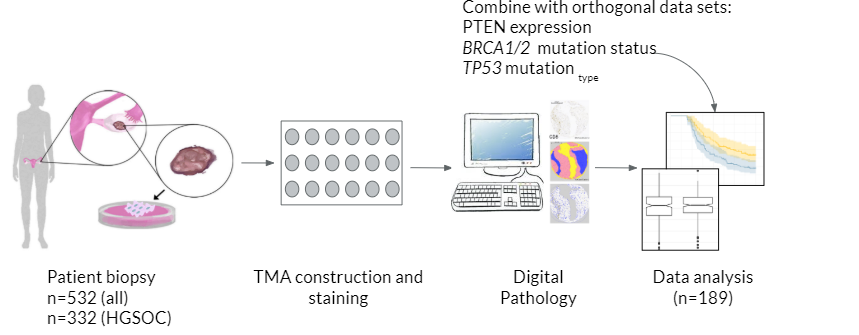
\includegraphics{Chapter2/Figs/Raster/Thesis_visual_abstract.PNG}
    \caption[Visual Abstract]{Visual abstract}
    \label{fig:visual_abstract}
\end{figure}

\section{SEARCH Cohort}

Samples from 570 patients from the prospective SEARCH ovarian cancer population-based study had been used to construct tissue microarrays. Ethical approval was granted by the Eastern Multicenter Research Ethics Committee. Among the samples from 570 patients with primary epithelial ovarian tumours, 332 were high grade serous ovarian cancer patients. All cases underwent detailed histopathological review by a gynaecological pathologist (JM). Patients were staged as having localized, regional or distant disease (L/R/D).

\section[Methods]{Methodology}
\subsection{SEARCH Data Set}
As mentioned, the immunohistochemical staining and initial utilization of Definiens software was carried out by AM. The methodology of all the data sets used in this section is outlined below and referred to in the Methods. 
\subsubsection{Immunohistochemistry}
Immunohistochemistry on the SEARCH samples was carried out upon the tissue sections by Anne Montfort (AM) according to the protocol in section \ref{sec:am_method}. Previously published PTEN immunostaining data was used where high PTEN expression was considered to be positive staining and low expression to be weak, heterogeneous or negative staining respectively\cite{RN17}.

\subsubsection{Mutation data}

Sequencing and mutation analysis was carried out prior to this PhD by Anna Piskorz (AP). The coding regions of TP53 were sequenced by tagged-amplicon next generation sequencing as previously described\cite{RN18} and confirmed by immunohistochemical analysis using a 4-tier core system\cite{RN19}. Sequencing of germline mutations in the  \texit{BRCA1} and \texit{BRCA2} genes was performed as previously described\cite{RN20}. Some samples were resequenced by SAK following my initial exploratory analysis and datacleaning steps. The results of resequencing were integrated into the final analysis.

\subsubsection{Immune cell quantification}
 The number of CD8$^+$ and CD45RO$^+$ cells in epithelial and stroma areas, the area of epithelial and stromal areas covered by CD68 staining and the total area of epithelium and stroma in each core, had been digitally determined using the Tissue Studio software (Definiens™).

Figure \ref{fig:segmentation} shows examples of the cell segmentation and tissue classification in the data set from this cohort.

\begin{figure}[htbp!] 
\centering    
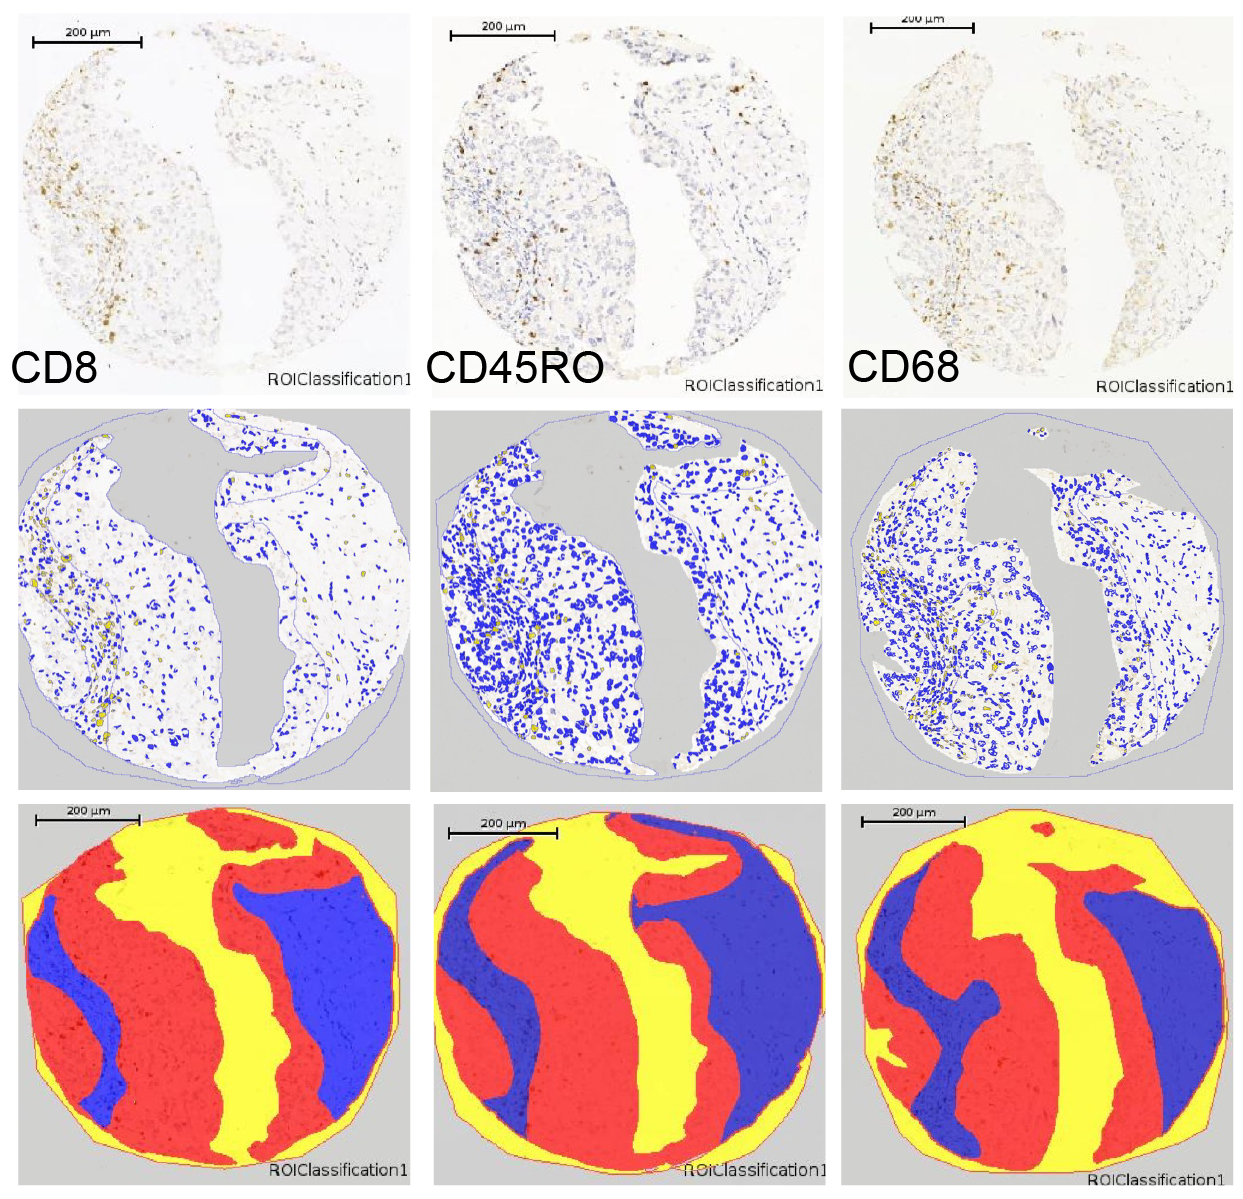
\includegraphics[width=0.8\textwidth]{Chapter2/Figs/Raster/Segmentation.png}
\caption[Segmentation in Definiens]{Examples of the segmentation of tissues and identification of cells in the Definiens software.}
\label{fig:segmentation}
\end{figure}

\subsection{Statistical analyses}
 The clinical variables of age at diagnosis, menopause status and stage were available for the cohort and I included them in the analysis. I used univariable Cox regressions to identify best-fitting variables for the final multivariable Cox regression model. The refined model was compared with a combined multivariable Cox regression model including all immune infiltrates. Hazard ratios (HR) refer to a single unit increase in continuous variables. The proportional hazards assumption was tested and satisfied in all cases using Schoenfeld residuals. The Kaplan–Meier analysis (with log-rank test) was applied to illustrate survival differences graphically. Two-sided P-values <0.05 were used to indicate statistical significance. 

Principal component analysis (PCA) using the R package prcomp was used to extract the independent components of variance between patients. The package prcomp uses singular value decomposition and the variables were scaled to have unit variance before creating composite linear independent variables. These were then passed forward to the survival modelling. The Akaike Information Criterion (AIC), equation \ref{eq:AIC} was used to compare the performance of survival models.

Bonferroni p-value corrections were carried out for all multiple testing. P < 0.05 was considered significant for all analyses. 


\section{Results}
 
As well as patients with High Grade Serous Ovarian Cancer, the SEARCH cohort included patients with Clear Cell, Endometrioid, Mucinous and Low Grade Serous Ovarian Cancer. These subtypes of Ovarian Cancer have vastly different cells of origin, different patterns of infiltration and different genomic drivers. As I was interested in understanding the differences within populations rather than across subtypes I extracted the HGSOC subpopulation for the initial analysis.

\subsection{Patient characteristics}
Figure {\ref{fig:remark_search}} shows the REMARK diagram for this study and Table \ref{table:clinical_SEARCH} shows the clinical characteristics of the 332 HGSOC patients from the study cohort. Immunohistochemical analyses on tissue microarrays (TMAs) were performed to detect CD8$^+$, CD45RO$^+$ and CD68$^+$ cells in tissue cores from primary ovarian specimens.  152 HGSOC cases were available for analysis after quality assurance, data cleaning and the reduction of the data set to only cases with complete results for CD8, CD45RO and CD68 staining in both epithelium and stroma as well as survival data. 
Tagged amplicon sequencing was performed on 248 cases and TP53 mutation was detected in 231 samples (93\%) (Table \ref{tab:clinical_SEARCH}). Previously published data for germline  \texit{BRCA1} and \texit{BRCA2} mutation and PTEN expression were available for 297 and 155 cases respectively\cite{17,20}.

\begin{figure}
    \centering
    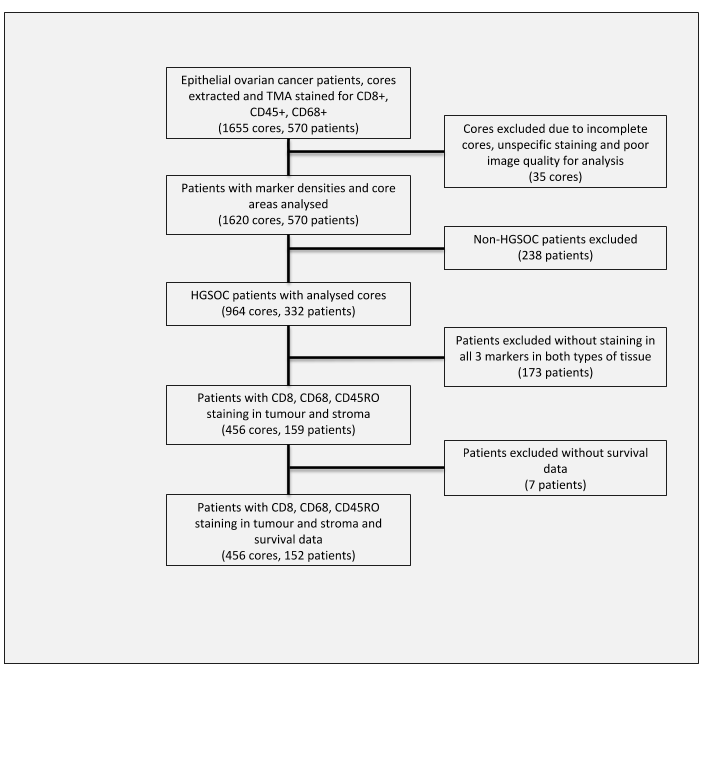
\includegraphics[width=0.8\textwidth]{Chapter2/Figs/Raster/montfort-REMARK.png}
    \caption{REMARK diagram for the SEARCH cohort.}
    \label{fig:remark_search}
\end{figure}
\begin{table}[]
    \centering
    \begin{tabular}{lll}
    \hline
 N	&	& 332 \\
Median Age (IQR) & & 58.0 (51.0-64.0) \\
\hline
Stage &	localized &	64 (19.3\%)\\
 &	regional &	42 (12.7\%)\\
 &	distant	& 202 (60.8\%)\\
 &	unstaged &	24 (7.2\%)\\
 \hline
TP53 mutation &	gof &	137 (55.2\%) \\
 &	lof &	94 (37.9\%)\\
&	wild type &	17 (6.9\%)\\
 &	Not assessed &	84 \\
 \hline
PTEN IF	& 	High &	28 (18.1\%)\\
& 	Low	 & 127 (81.9\%)\\
&	Not available &	177 \\
\hline
BRCA status		& 	wild type &	256 (86.2\%)\\
 &	\textit{BRCA1} &	18 (6.1\%)\\
 &	\texit{BRCA2} &	23 (7.7\%)\\
 &	Not available &	35\\
\hline
    \end{tabular}
    \caption{Patient characteristics for the HGSOC subset of the SEARCH cohort.}
    \label{tab:clinical_SEARCH}
\end{table}

 \subsection{Data cleaning, quality assurance and spatial bias}

One of the valuable things about analysing a large number of digitally imaged and segmented TMA cores is the ability to carry out quality checking for bias across TMAs and to evaluate the impact of and the variation in properties of the tissue core such as tissue area, something not measured by pathologists when assessing cores manually.

I examined the distribution of tissue area and ensured that the varying tissue area across TMAs was random. I did this visually using heatmaps (Figure \ref{fig:heatmap_area}) and statistically using Shapiro-Wilk tests ($p > 0.05 $). 

\begin{figure}
    \centering
    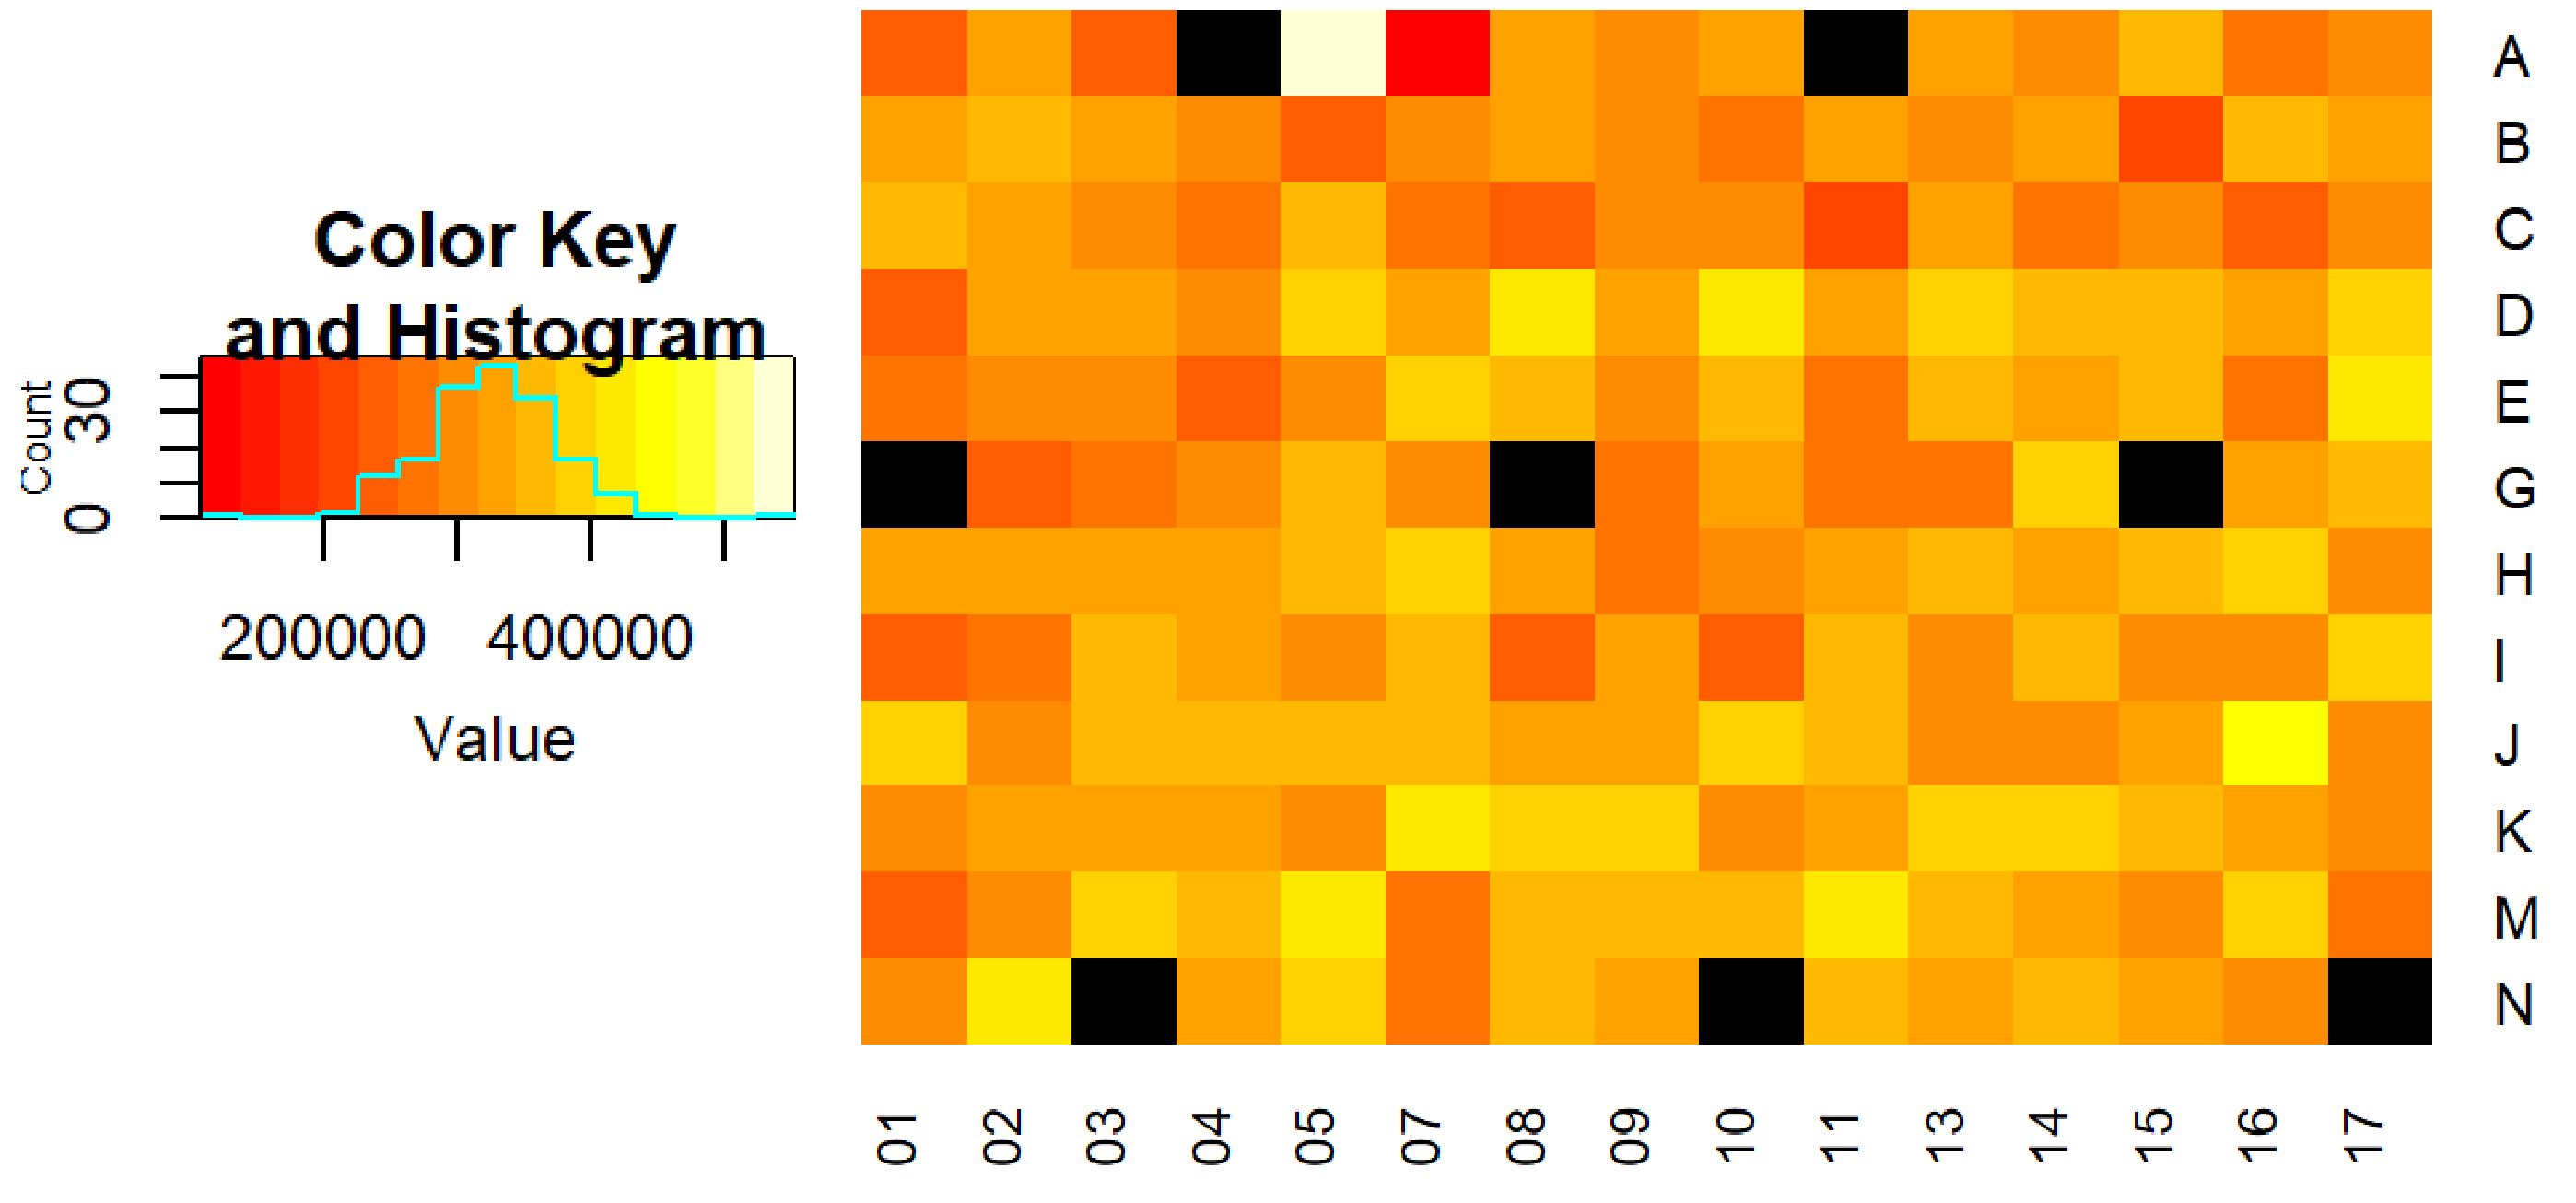
\includegraphics[width=0.8\textwidth]{Chapter2/Figs/Raster/area_heatmap.png}
    \caption{Heatmap of total core area across TMA.}
    \label{fig:heatmap_area}
\end{figure}


 
As mentioned, CD8+ and CD45RO+ counts were initially calculated as number of cells in stroma and epithelium and CD68+ scoring was given as area covered. I processed this raw data, converting cell counts into cells per unit area and CD68+ coverage into percentage area. This area normalization allows for comparison between cores and patients whose tumour tissue is made up of varying quantities of stroma and epithelium. 

I also extracted outlying examples of cores to ensure the despite the tissue area sampled varying, that the measures of infiltrate density were not significantly different from the population as a whole. Figure \ref{fig:heatmap} shows a heatmap comparing infiltration density across the CD8$^+$ , CD68$^+$ and CD45RO$^+$ TMAs. No spatial relationship was observed over a single TMA between the location of a core and the density of immune cells or the tissue area. 



\begin{figure}
    \centering
    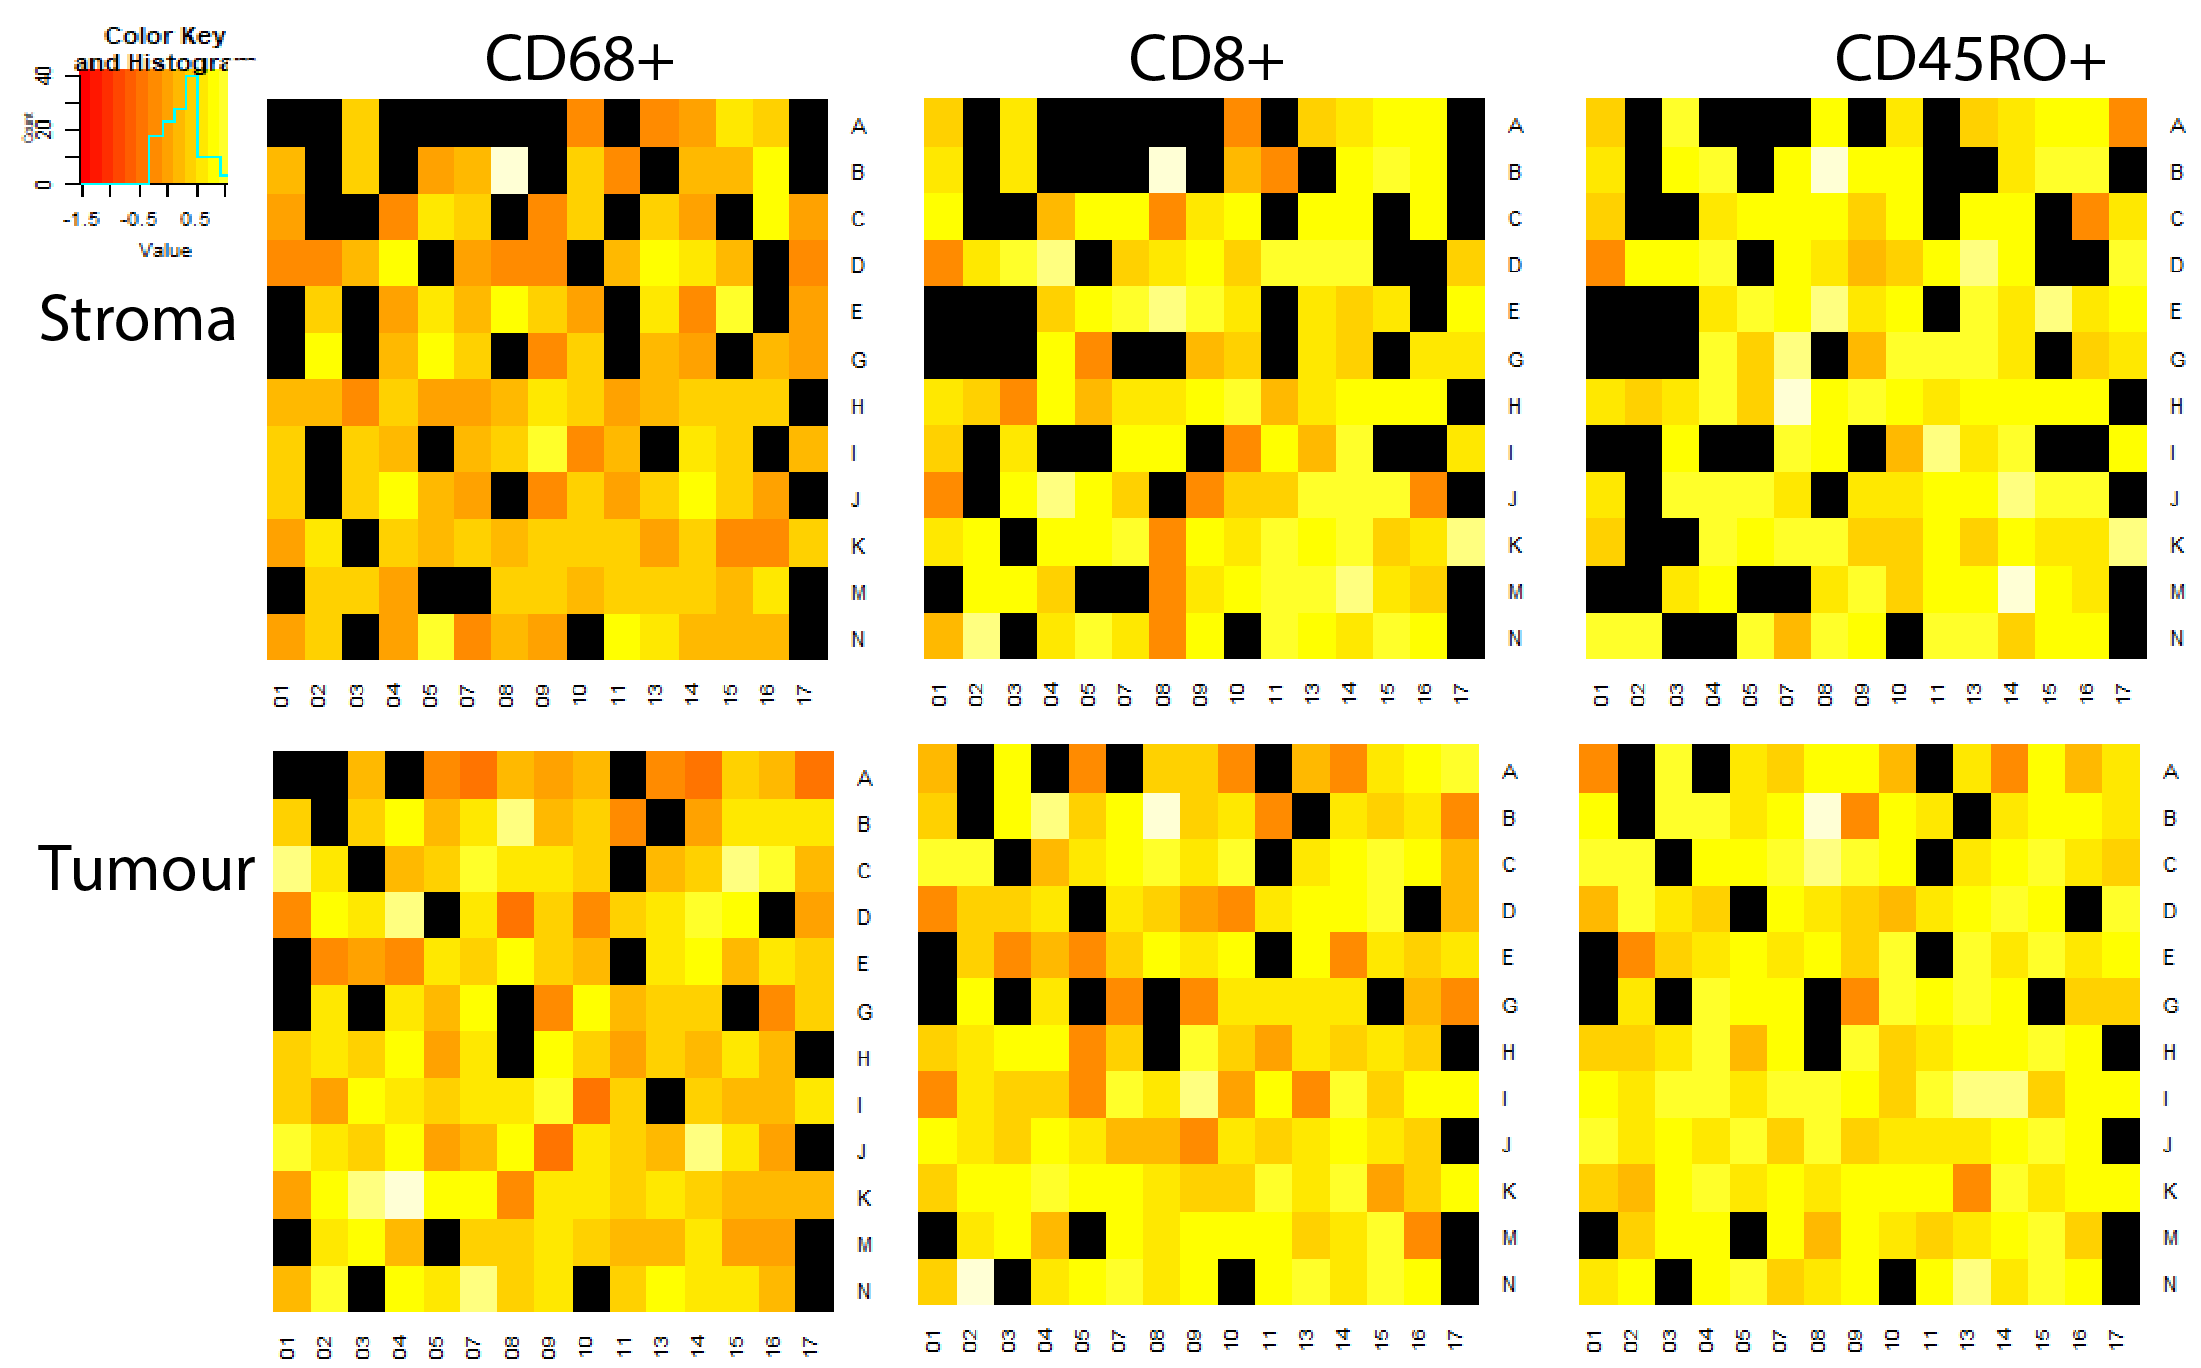
\includegraphics{Chapter2/Figs/Raster/Thesis-heatmap.png}
    \caption{Density of each infiltrate for each position in the SEARCH TMA.}
    \label{fig:outlying_core}
\end{figure}


\subsection{Stroma and tumour composition of cores}
As described in the methods, image analysis software (Definiens) was previously used to segment images of cores to determine the area of tumour epithelium and stroma in each core, this segmentation is shown in Figure \ref{fig:segmentation}. The distribution of tumour and stroma areas are shown in Figure \ref{fig:distribution_infiltrate}A. Digital pathology and tissue segmentation provides a unique opportunity to evaluate stromal and epithelial areas and the makeup of sampled tissue cores. The sampling of tissue from a tumour for the construction of TMAs is usually aimed towards extracting epithelium and I wanted to investigate how these TMAs had sampled tumour and stromal tissue. I initially investigated the epithelial and stromal composition of the core images and found that of 964 images representing 332 HGSOC patients, 69 patients (20.8\%) had images which contained malignant epithelium but no stroma; 250 patients (75.3\%) had images which contained epithelium and >1\% adjacent stroma and 13 patients (3.9\%) had images containing no tumour epithelium (Fig \ref{fig:distribution_infiltrate}A). The median proportion of epithelium and stroma was 85.1\% (IQR 51–100\%) and 14.9\% (IQR 0–49\%) respectively.



I was interested in whether the percentage of tumour in a core was correlated with the \textit{p53} mutant allele fraction measured through sequencing for the patient. As p53 mutations are found ubiquitously in HGSOC tumour cells we expect the proportion of tumour in a sample to be correlated with p53 mutant allele fraction although the sequencing and sectioning are not carried out on exactly the same tumour region. I found them to be positively correlated ($R= 0.24$, $p=0.0027$). The correlation between technical replicates for allele frequency and sequencing depth is shown in Appendix \ref{fig:p53_allele}. 
\begin{figure}
    \centering
    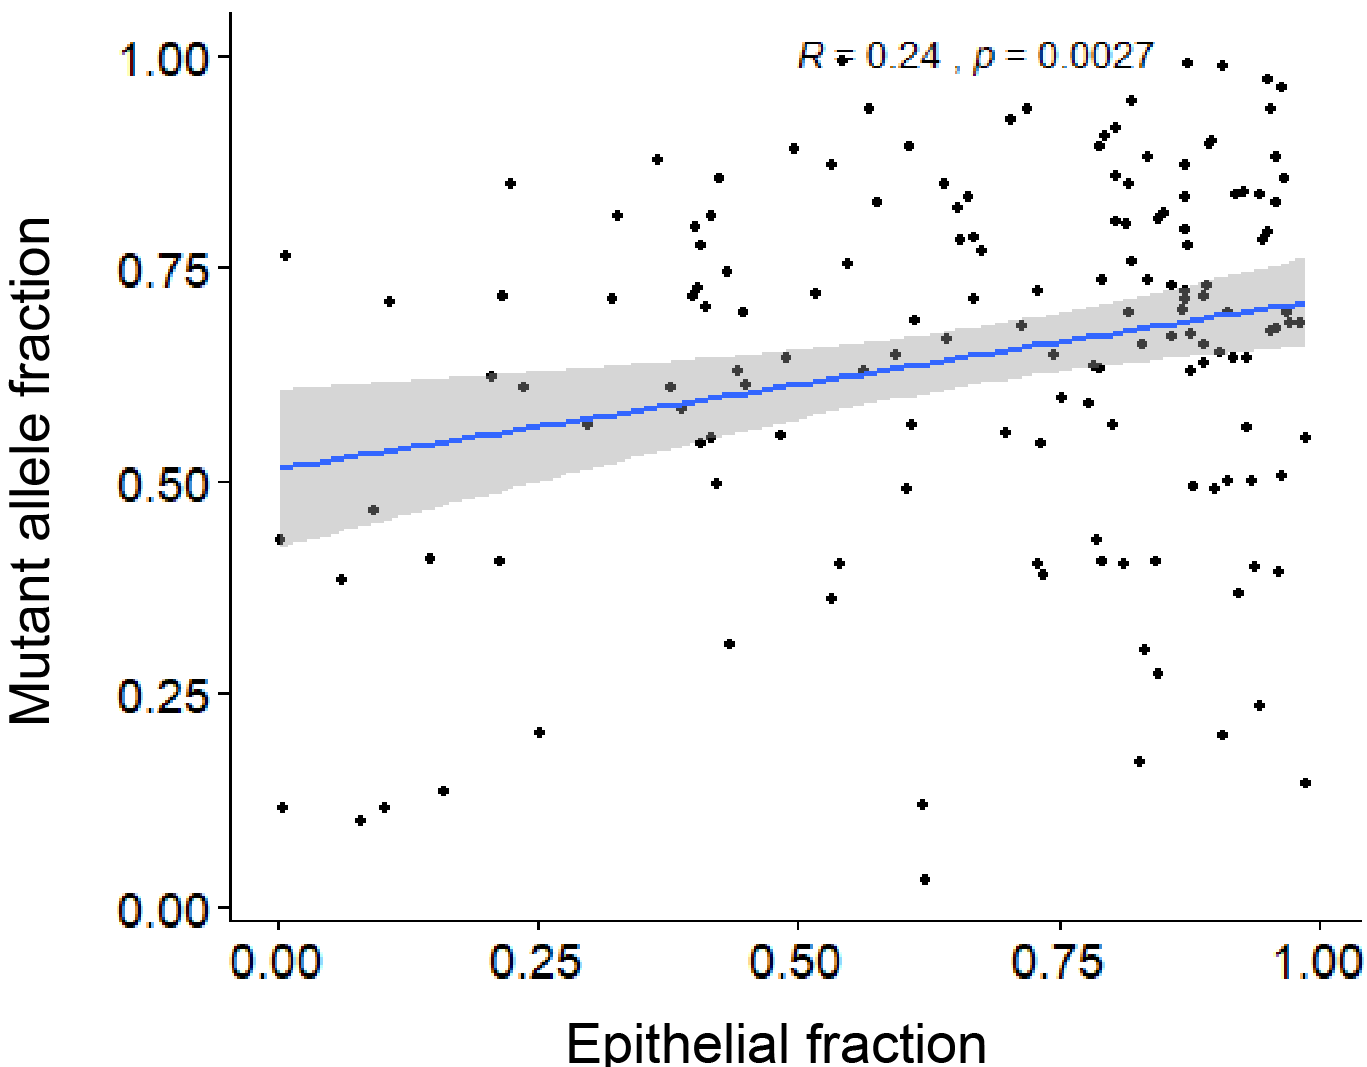
\includegraphics{Chapter2/Figs/Raster/maf_epithelial.png}
    \caption{\textit{p53} mutant allele fraction against epithelial area of a core.}
    \label{fig:p53_allele}
\end{figure}

I also examined the mutant allele fraction across samples (Figure \ref{fig:maf_dist} to ensure that the samples were HGSOC and to investigate whether all samples were of high enough quality. Samples with mutant allele fraction of zero were resequenced and if no mutation was found were excluded from HGSOC analysis.
\begin{figure}
    \centering
    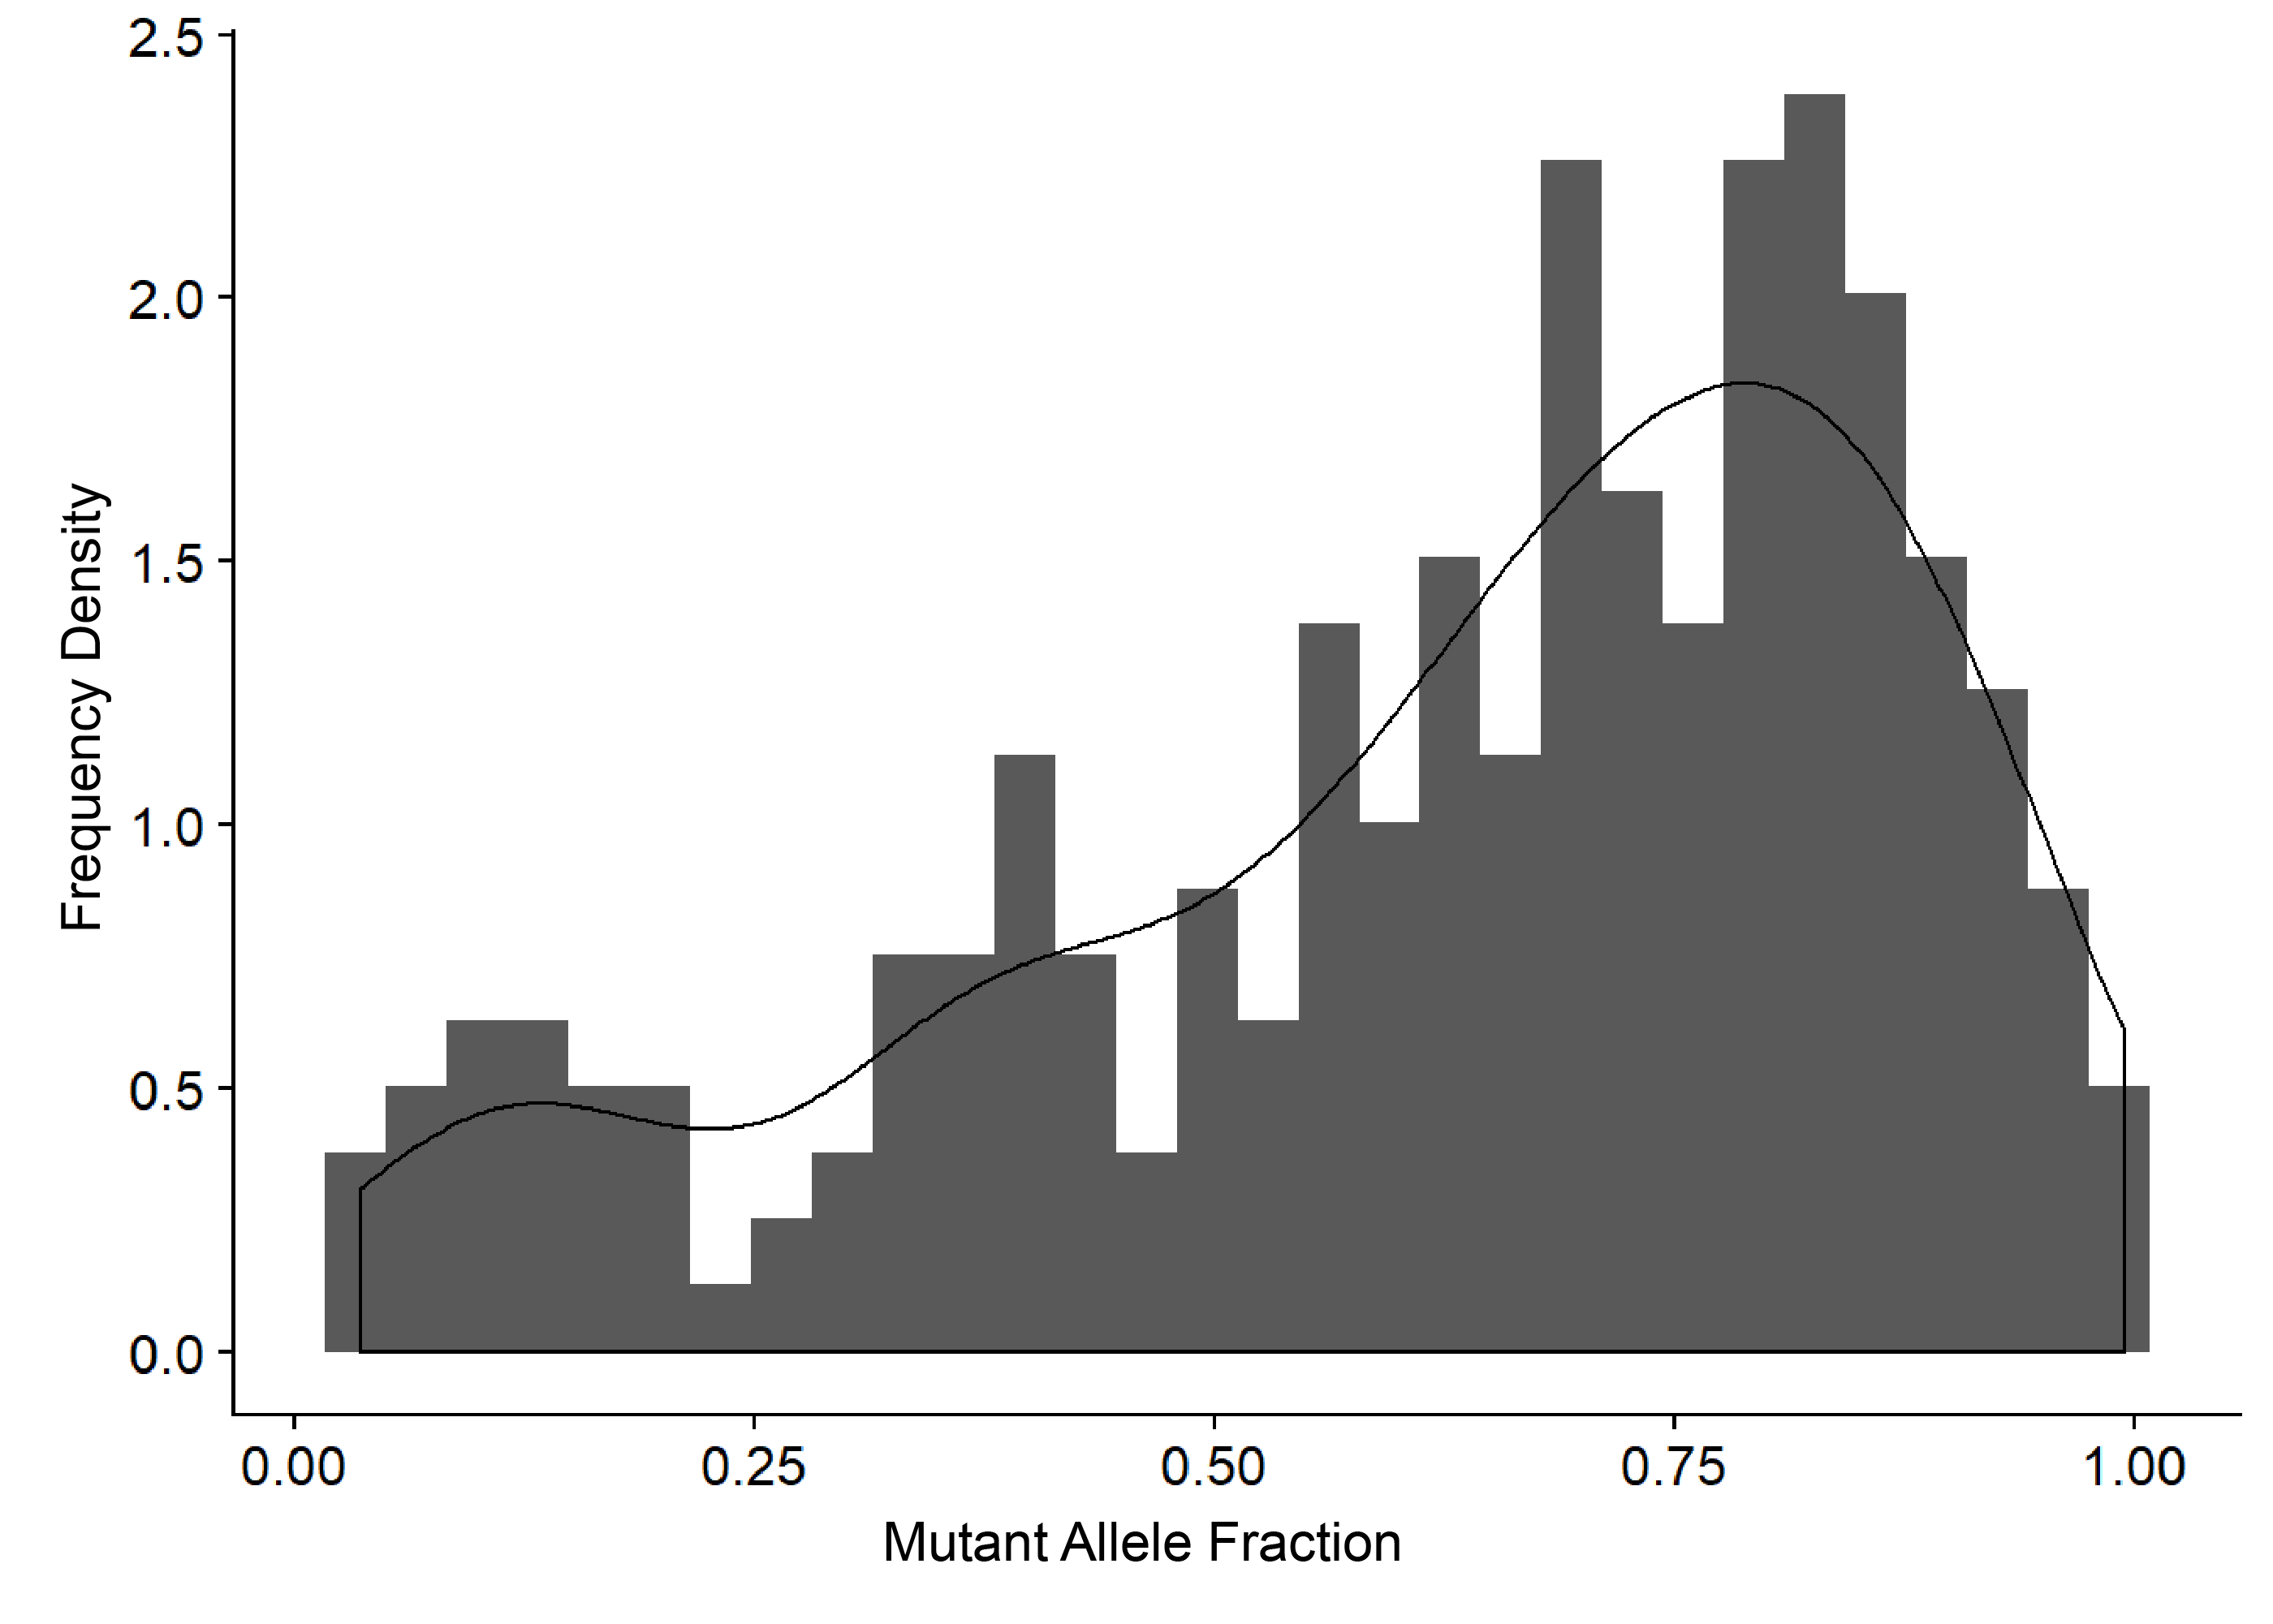
\includegraphics[width=0.4\textwidth]{Chapter2/Figs/Raster/MAF_distribution.png}
    \caption{Histogram of counts of samples against mutant allele fraction.}
    \label{fig:maf_dist}
\end{figure}


\subsection{Immune cell densities}


As mentioned, cell counts of all immune populations were generated by a collaborator and pathologist through Definiens software. An example of the assessment of CD8$^+$ T cell, CD45RO$^+$ memory lymphocyte and CD68$^+$ macrophage densities and the allocation of the stromal and epithelial compartment that was obtained are shown in Fig. \ref{fig:segmentation}.

When looking at the overall infiltration of a sample and the survival impact, without segmenting the cores, this means that you are measuring both the stromal and epithelial infiltrate. I felt that it was important to know whether the density of infiltration varied between epithelial and stromal compartments. The distribution of densities of immune populations within tumour epithelium and stromal areas were compared (Fig. \ref{fig:distribution_infiltrate}B–D). The density of CD8$^+$ and CD45RO$^+$ cells were significantly higher in stroma than tumour epithelium (p = 0.005 and p = 0.004 respectively; Welch’s t-test) but not significantly different for CD68$^+$ cells. 

\begin{figure}
    \centering
    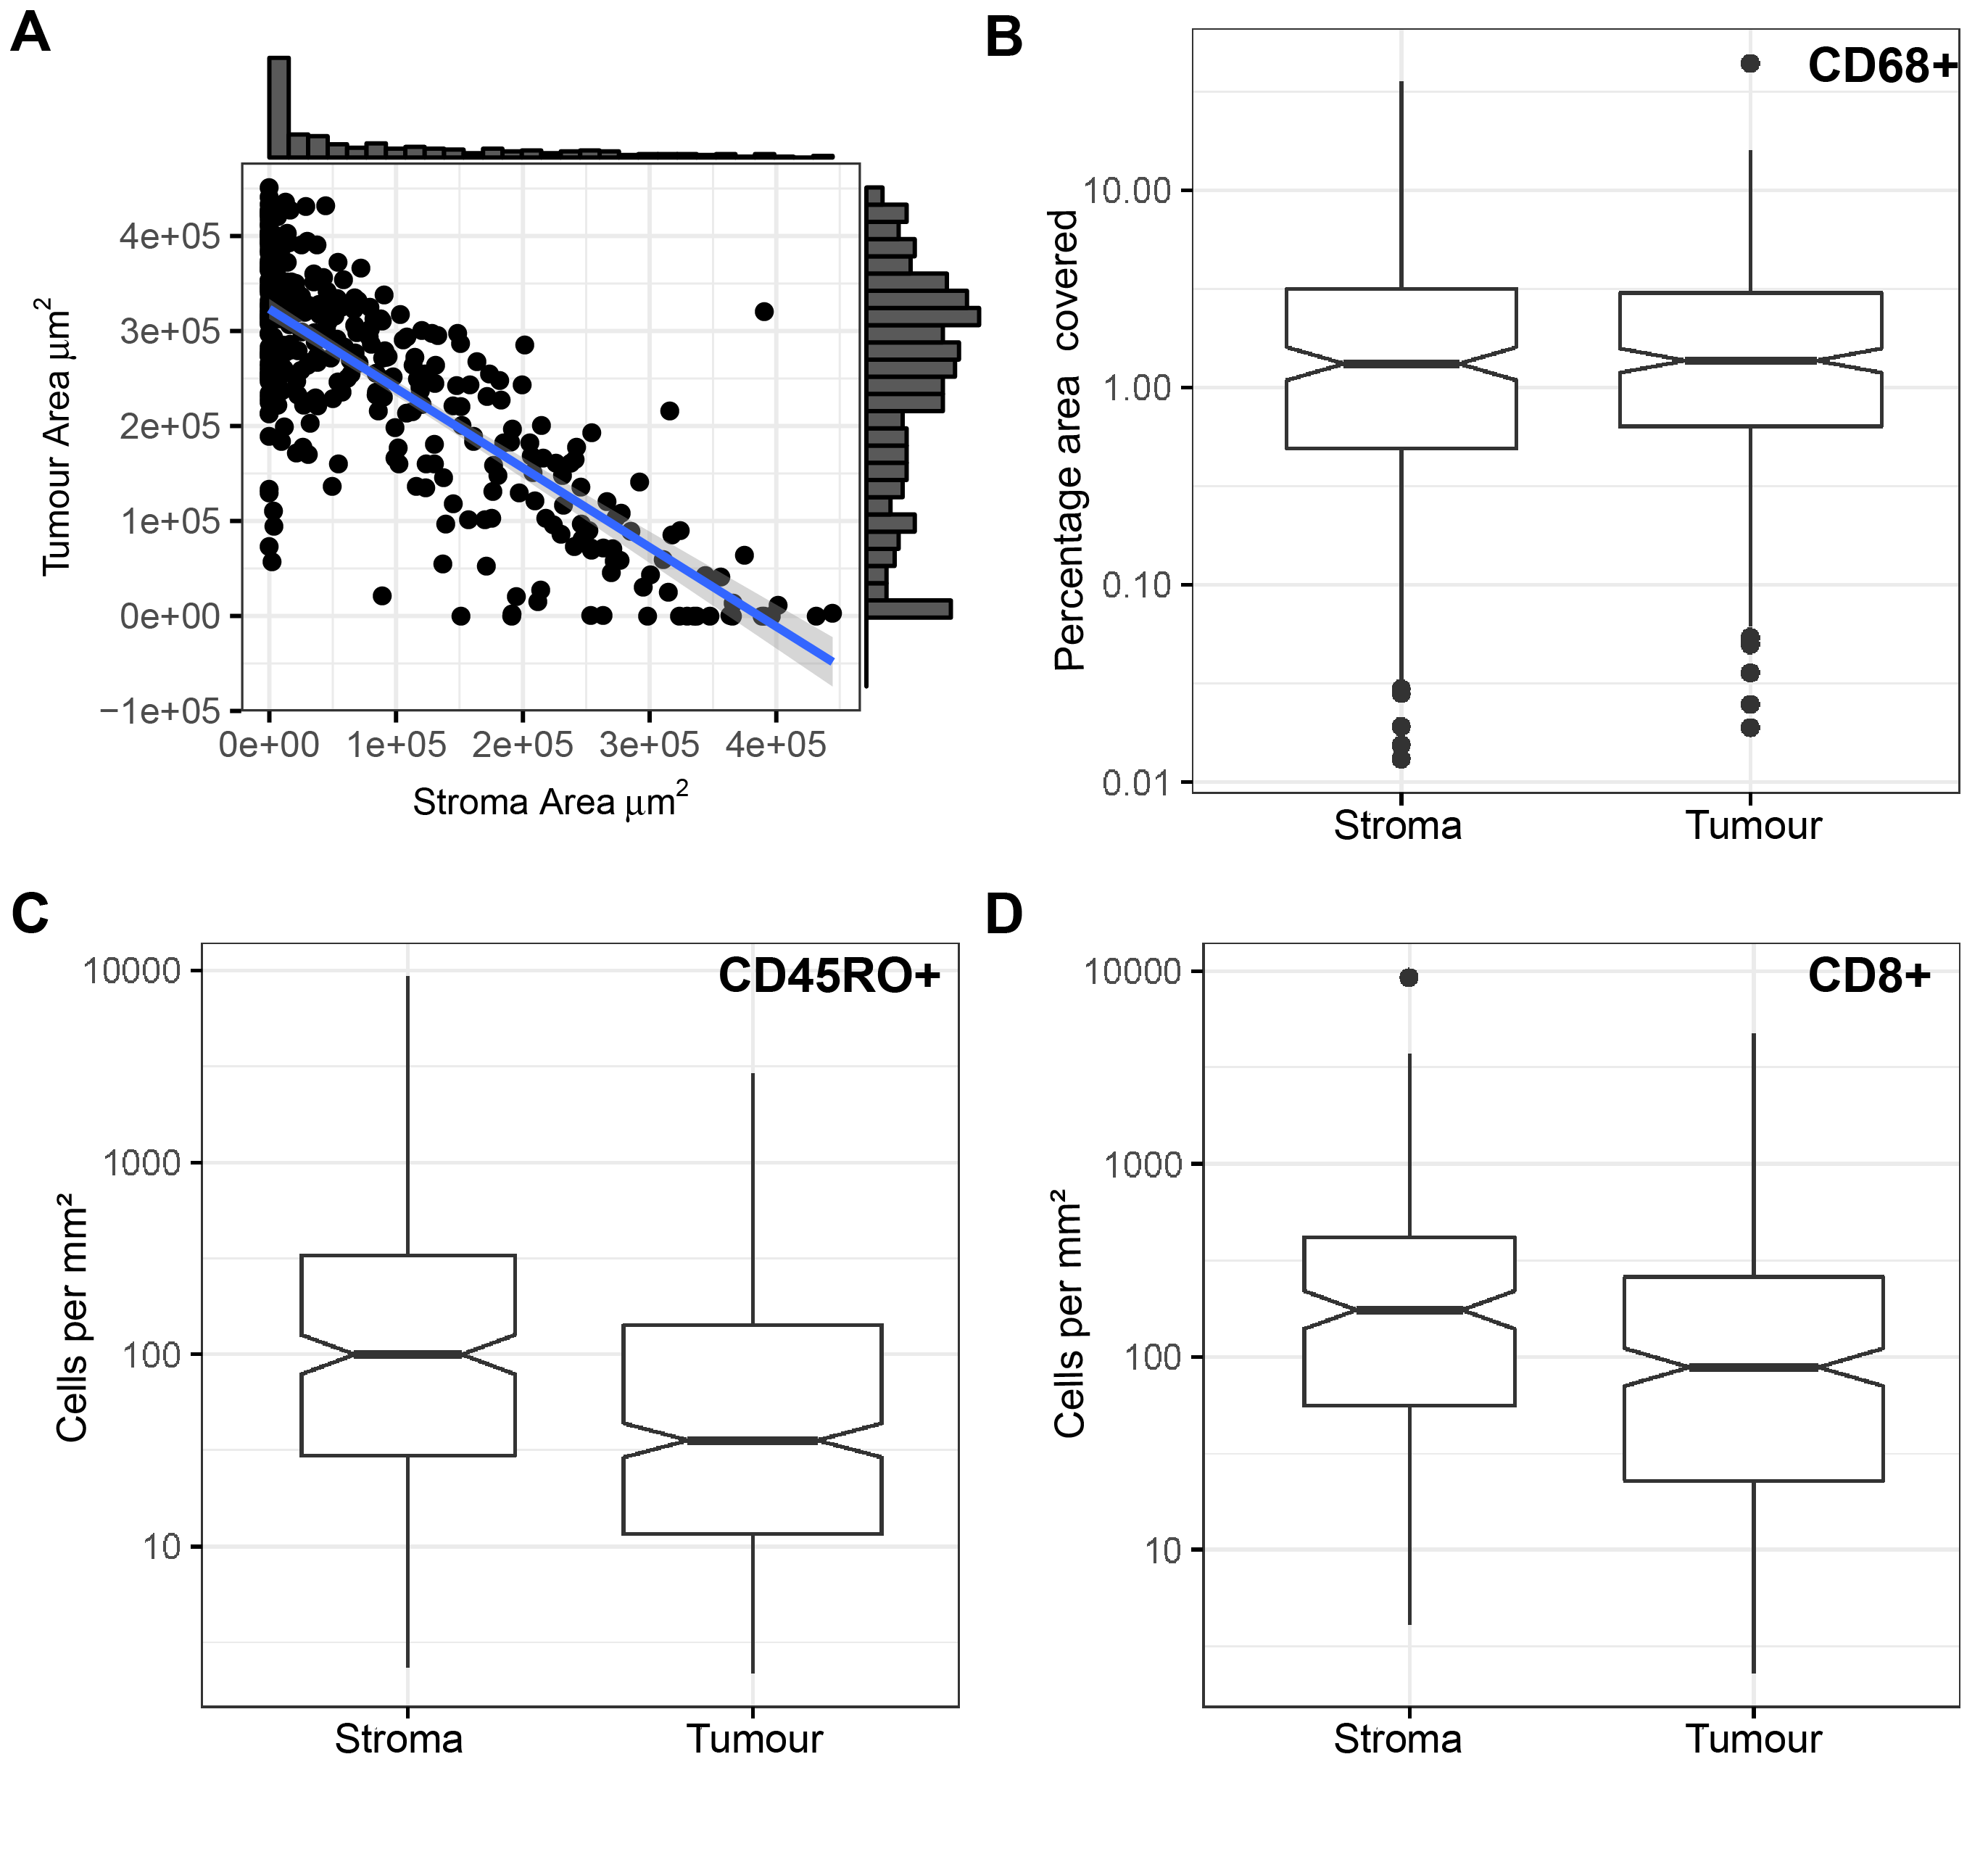
\includegraphics[width=0.8\textwidth]{Chapter2/Figs/Raster/plots_dist.png}
    \caption[Distribution of immune densities.]{ (A) Scatter plot of the stroma and epithelial  areas averaged across sections for each patient. (B), (C) and (D) show the distribution of immune cell densities in epithelium and stroma. CD8$^+$ and CD45RO$^+$ densities were defined as counts per mm2 and CD68$^+$ as the percentage of tissue stained for this marker. (Notches on box plots extend 1.58 ✕ IQR / sqrt(n) and approximate the 95\% confidence interval for the median. Box plot whiskers extend to 1.5 ✕ IQR.) 
}
    \label{fig:distribution_infiltrate}
\end{figure}

Another major direction in the literature is the focus on epithelial CD8$^+$ infiltrate, I was interested in whether this infiltrate is independent of others or whether this infiltrate is also an indirect readout of other infiltrates which may also have impacts on the patient. This is as well as the correlation between infiltrates being important to understand whether there exist spatial dynamics of infiltration and its movement between compartments. The three immune populations in our samples showed moderate to strong correlation between the infiltrate in epithelium and stroma and between each other (Figure \ref{fig:ch2_correlation} and Table \ref{tab:cor_pvals}). This means that samples with low density of stromal immune populations generally had low density of epithelial infiltrate and vice versa. It also meant that patients with high quantities of one infiltrate type often had high infiltration of the others.

\begin{figure}
    \centering
    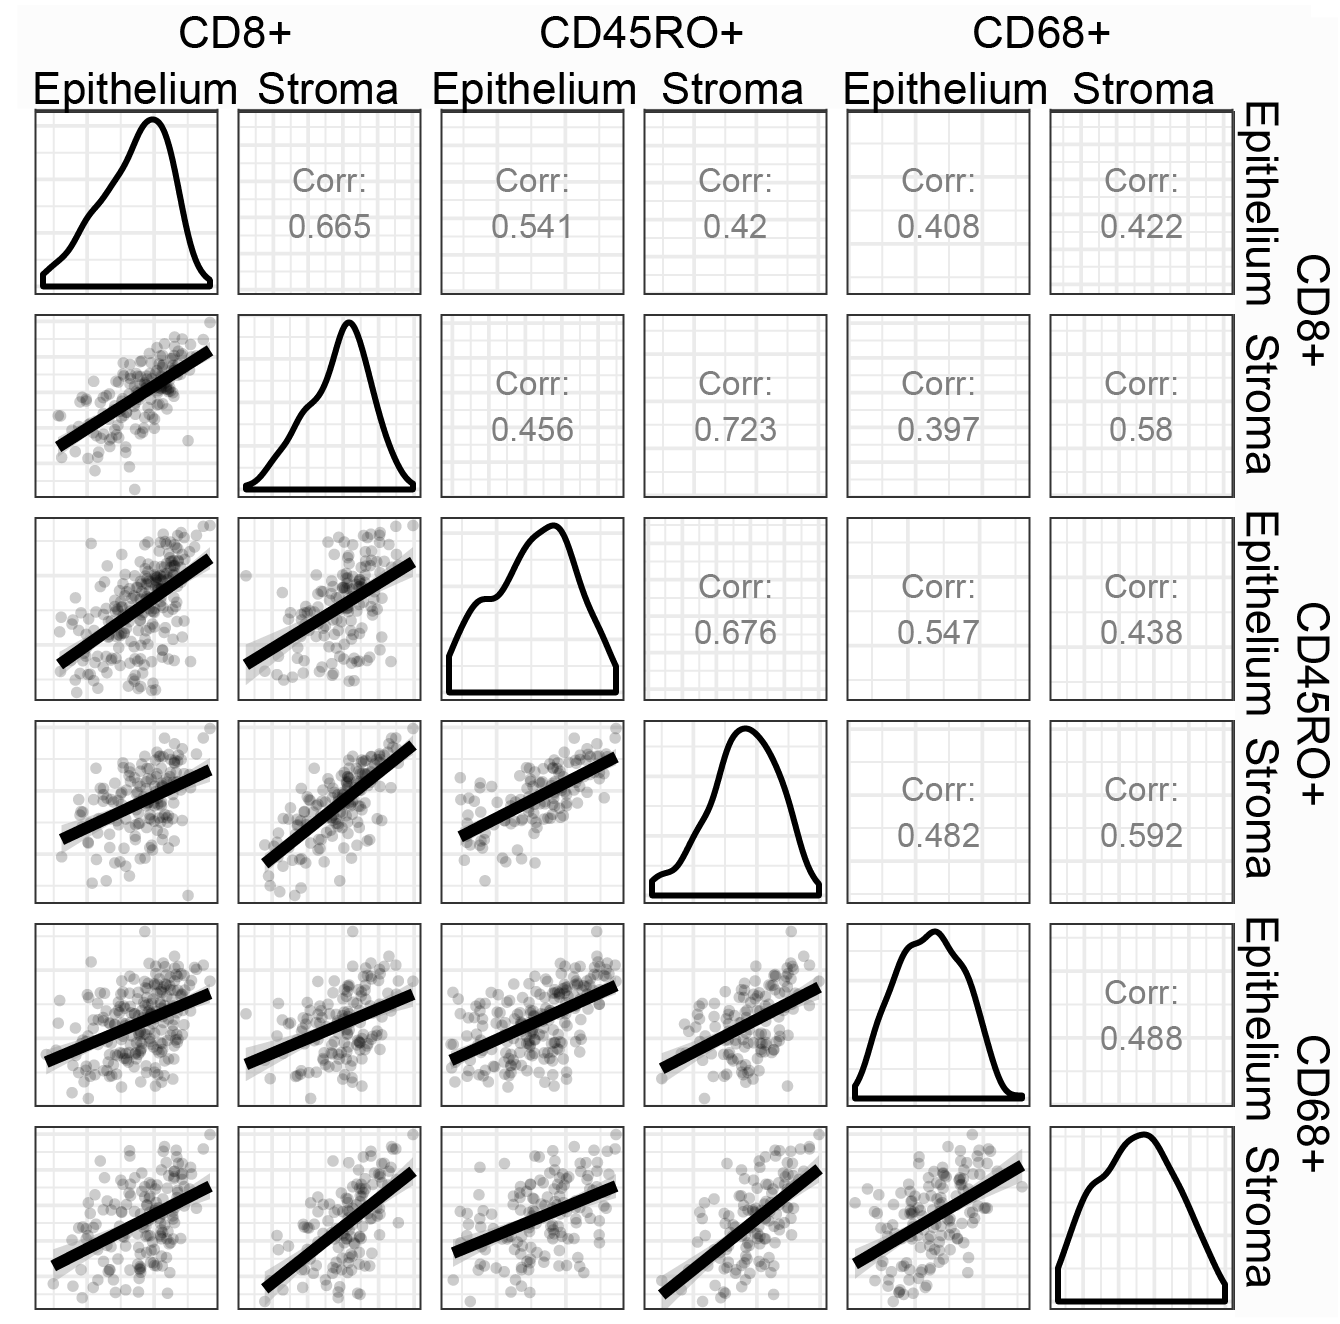
\includegraphics[width=0.8\textwidth]{Chapter2/Figs/Raster/correlation_inf.png}
    \caption[Correlation between infiltrates]{Scatterplots and distributions of CD68$^+$, CD45RO$^+$ and CD8$^+$ infiltrate in Stroma and Epithelium. All infiltrates were correlated between matched samples across both tissue region classes.}
    \label{fig:ch2_correlation}
\end{figure}

Given that we see varying tumour percentages and increased infiltrate in the stroma as compared with the tumour I was interested in whether the density of immune infiltrate reaching the epithelium was related to the epithelial percentage of the core. In  other words, does increasing the quantity of tumour in a sample increase the infiltration, perhaps due to the presence of more tumour antigens and immune cell recruitment or decrease it due to reduced stromal access and infiltration. I examined the relationship between the fraction of tumour in a core and the density of immune infiltration in the epithelium using Pearson correlation test. Intra-epithelial CD8$^+$ and CD45RO$^+$ densities were  weakly positively correlated with the purity/tumour fraction of the sample ($R^2 = 0.17$, $p = 0.003$ and $R^2 = 0.16$, $p=0.006$) whereas CD68$^+$ epithelial density was not.



\subsection{Immune exclusion}

When considering patterns in immune infiltration, beyond the binary of present and absent, the terms immune-inflamed, immune-desert and immune-excluded have been used to describe varying T-cell infiltration based on histological and transcriptional analyses \cite{}. Immune-inflamed and immune-desert patterns reflect high positive or negative correlations between all infiltrates but T-cell exclusion describes tumours where CD8$^+$ cells are significantly absent from tumour epithelium whilst still being present in the surrounding stroma\cite{26,27}. 

Given the higher infiltration in stroma than epithelial compartments,. I expect to see XYZ, therefore I defined immune cell exclusion as a 10-fold difference between tumour epithelium and stromal infiltration as the standard deviation of the log10 transformed counts was approximately 1. CD8$^+$ exclusion was present in 20 (10.6\%) cases and 36 (20\%) cases had CD45RO$^+$ exclusion. No cases had significant exclusion of CD68$^+$ infiltrate from tumour epithelium.  Notably despite 10 and 20\% of patients having CD8$^+$ and CD45RO$^+$ exclusion, none of the cases had both CD8$^+$ and CD45RO$^+$ exclusion. %Expand on why I used 10 fold cut off etc, examine cutoffs etc and differences. INCLUDE PLOT.



\subsection{Functional form of infiltrates in building a survival model}
When modelling survival using Cox regression, one must decide upon the functional form of the predictor\ref{eq:cox}.  In order to find the best functional form for each predictor I modelled the univariate relationship between the predictor and survival using Cox regression and plotting the residuals of the model fit against the expected form. The relationship between each of the immune variables and survival was found to be approximately log-linear. The only clinical variables accompanying the cohort were age at diagnosis, stage and menopause status. Age at diagnosis is the only continuous variable of these and the relationship between age and survival was found to be approximately linear (Figure \ref{fig:modelfit}, Supplementary Table \ref{tab:model_fit}). 

\begin{figure}
    \centering
    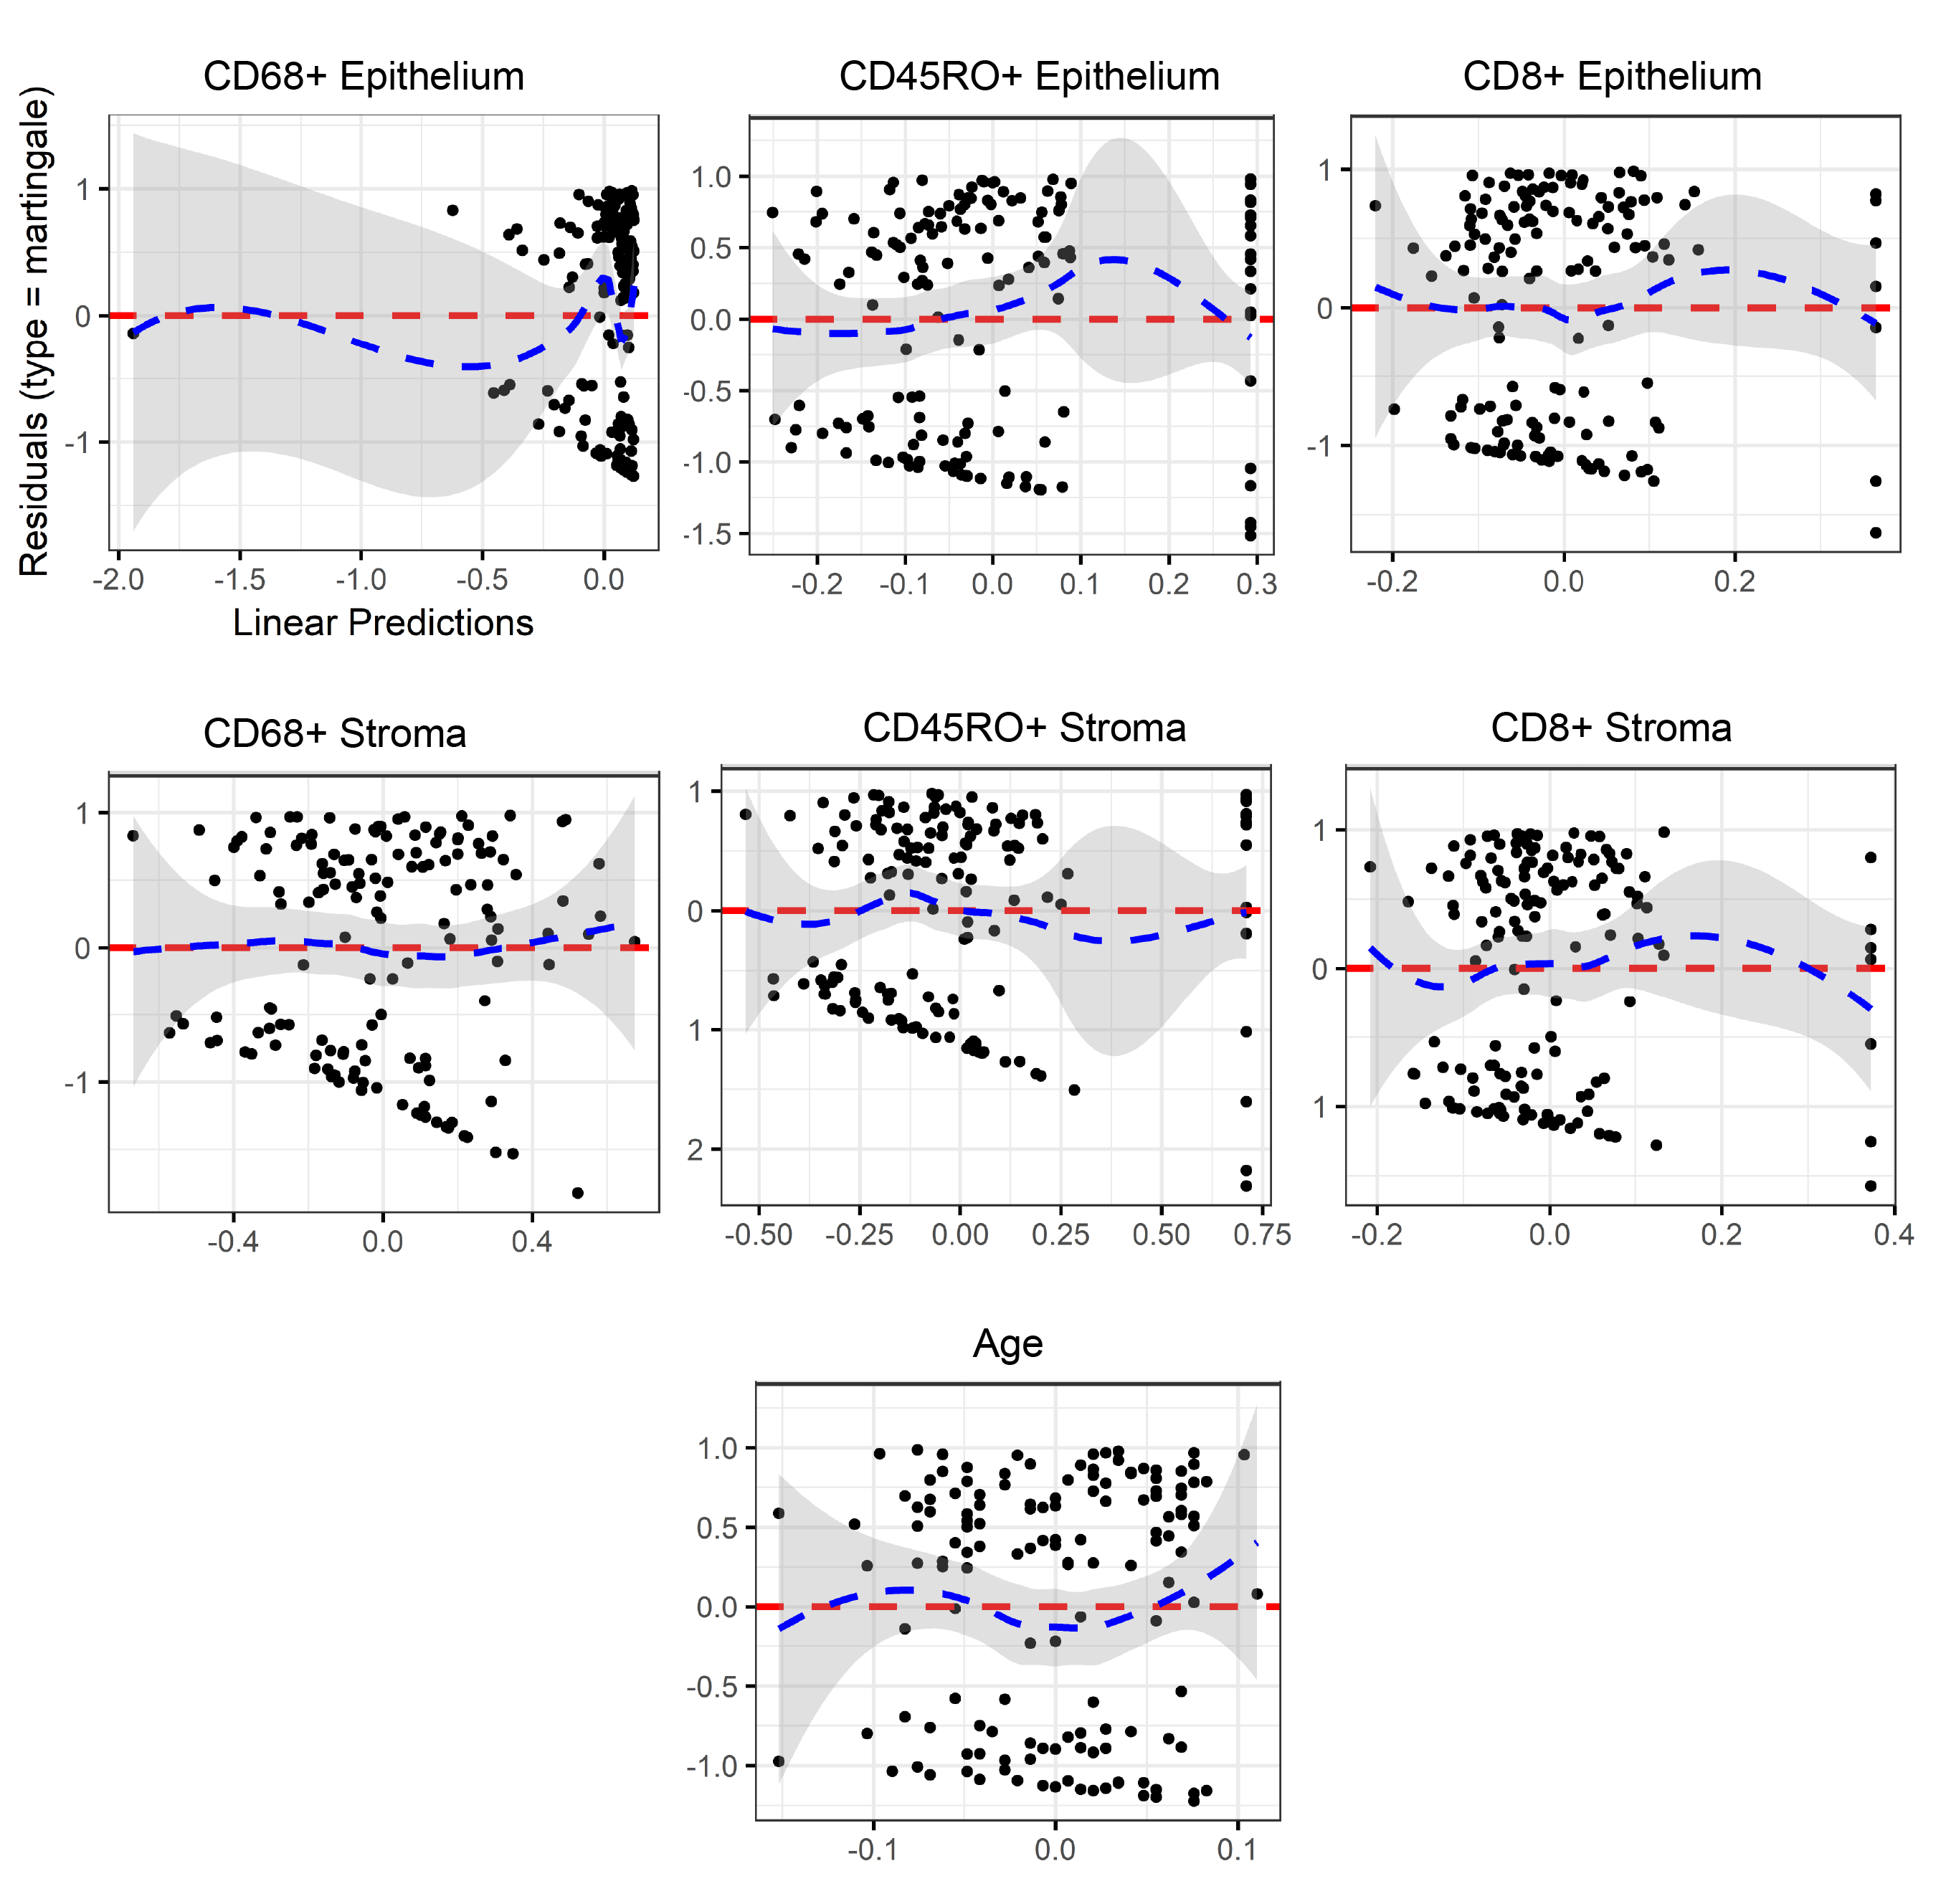
\includegraphics[width=\textwidth]{Chapter2/Figs/Raster/modelfit_2-08.png}
    \caption[Residuals of model fit]{Residuals of model fit plotted against predicted value for log-transformed immune variables and age at diagnosis. All relationships were found to be approximately linear.}
    \label{fig:modelfit}
\end{figure}



\subsection[Prognostic value of individual infiltrates]{Stromal CD68$^+$ and CD45RO$^+$ infiltrate are the strongest individual prognostic markers}

Initially I investigated survival models of individual infiltrates in stroma and tumour. Univariable analysis showed improved survival with increasing stromal density of CD45RO$^+$ (HR 0.76 95\% CI 0.65–0.90, p=0.001) and CD68+(HR 0.53 95\% CI 0.34–0.81, p=0.003) (Table \ref{tab:coxsurv}). Modelling each immune variable with stage showed improved predictive value for epithelial CD8$^+$ density (HR=0.83, p-value=0.027) as well as stromal CD68$^+$ and CD45RO$^+$ density and epithelial CD45RO$^+$ density (Table  \ref{tab:coxsurv}). Kaplan-Meier curves have an arbitary cutpoint for continuous data and so I used these for illustrative purposes only. Figure \ref{fig:kmcd68845}) shows illustrative Kaplan-Meier survival curves for high and low stromal and epithelial CD68$^+$, CD45RO$^+$ and CD8$^+$ densities.\\

As I reduced my analysis to examine cores that contained tumour and stroma, my analysis is biased towards immune impact in a stromally infiltrated environment, I wanted to test whether CD45RO$^+$ and CD8$^+$ infiltrate were still significant predictors in predominantly epithelial cores. In the separate subset of cores with <1\% stroma, epithelial CD8$^+$ malignant epithelial infiltrate remained an independent prognostic factor but epithelial CD45RO$^+$ density was not significant (n=, Table \ref{tab:surv_cd8_epi}). %KEY DISCUSSION POINT

\subsection{Averaging immune infiltrate over a core}

In clinical reporting, quantifying immune populations in exclusively tumour epithelium is technically challenging and time consuming. I was therefore interested in testing the value of using the average density of each marker averaged across both tumour and stromal regions from each core (Table 1).  Averaging the tissue density of CD8$^+$ increased the strength of the associated hazard ratio and significance of the model (HR=0.79, p-value=0.010) indicating increased prognostic value for CD8$^+$ infiltrate over quantitation of individual epithelial and stromal infiltrates. The significance did not increase for CD45RO$^+$ and CD68$^+$ infiltrates.  Figure \ref{fig:KM_infiltrates} shows illustrative Kaplan-Meier survival curves for high and low CD68$^+$, CD45RO$^+$ and CD8$^+$ densities over combined epithelium and stroma compartments.\\


\begin{landscape}
\begin{table}[]
    \centering
    \begin{tabular}{llllllll}
    
		& & &&		Univariable && \multicolumn{2}{c}{	Multivariable* 
(adjusted for stage)} \\
								
&	Functional Form &	Evaluable cases&	Tissue compartment&	HR &	p-value	& HR &	p-value	\\ \hline
CD8$^+$&	log10 &	301	&Epithelium&	0.89&	0.15&	0.83&	0.027\\	
&	log10&	202&	Stroma&	0.97&	0.74&	0.93&	0.40\\	
&	log10&	315&	Average&	0.79&	0.010&	0.72&	0.0006\\	
CD45RO+&	log10&	290&	Epithelium&	0.86&	0.033&	0.85&	0.022\\	
	&log10&	196&	Stroma&	0.76&	0.001&	0.76&	0.0007\\	
	&log10&	306&	Average&	0.82&	0.006&	0.80&	0.003\\	
CD68+&	linear&	293&	Epithelium&	0.99&	0.67&	0.99&	0.43\\	
&	log10&	226	&Stroma	&0.53&	0.003&	0.44&	0.0003	\\
&	log10&	308	&Average&	0.67&	0.042&	0.62&	0.017\\	
Stage1 & - &	312&	Localised&	1&	0&	1&	0	\\
	& & &		Regional&	1.47&	0.26&	1.15&	0.25\\	
	&	&&	Distant	&3.96&	<<0.001&	5.58&	<<0.001	\\
	&	&&	Unstaged&	3.35&	<0.001&	3.34&	<<0.001	\\ \hline

\end{tabular}
    \caption[Individual immune infiltrates Cox regression]{Cox proportional hazards survival analysis for individual infiltrates.}
    \label{tab:coxsurv}
\end{table}
\end{landscape}

\begin{figure}
    \centering
    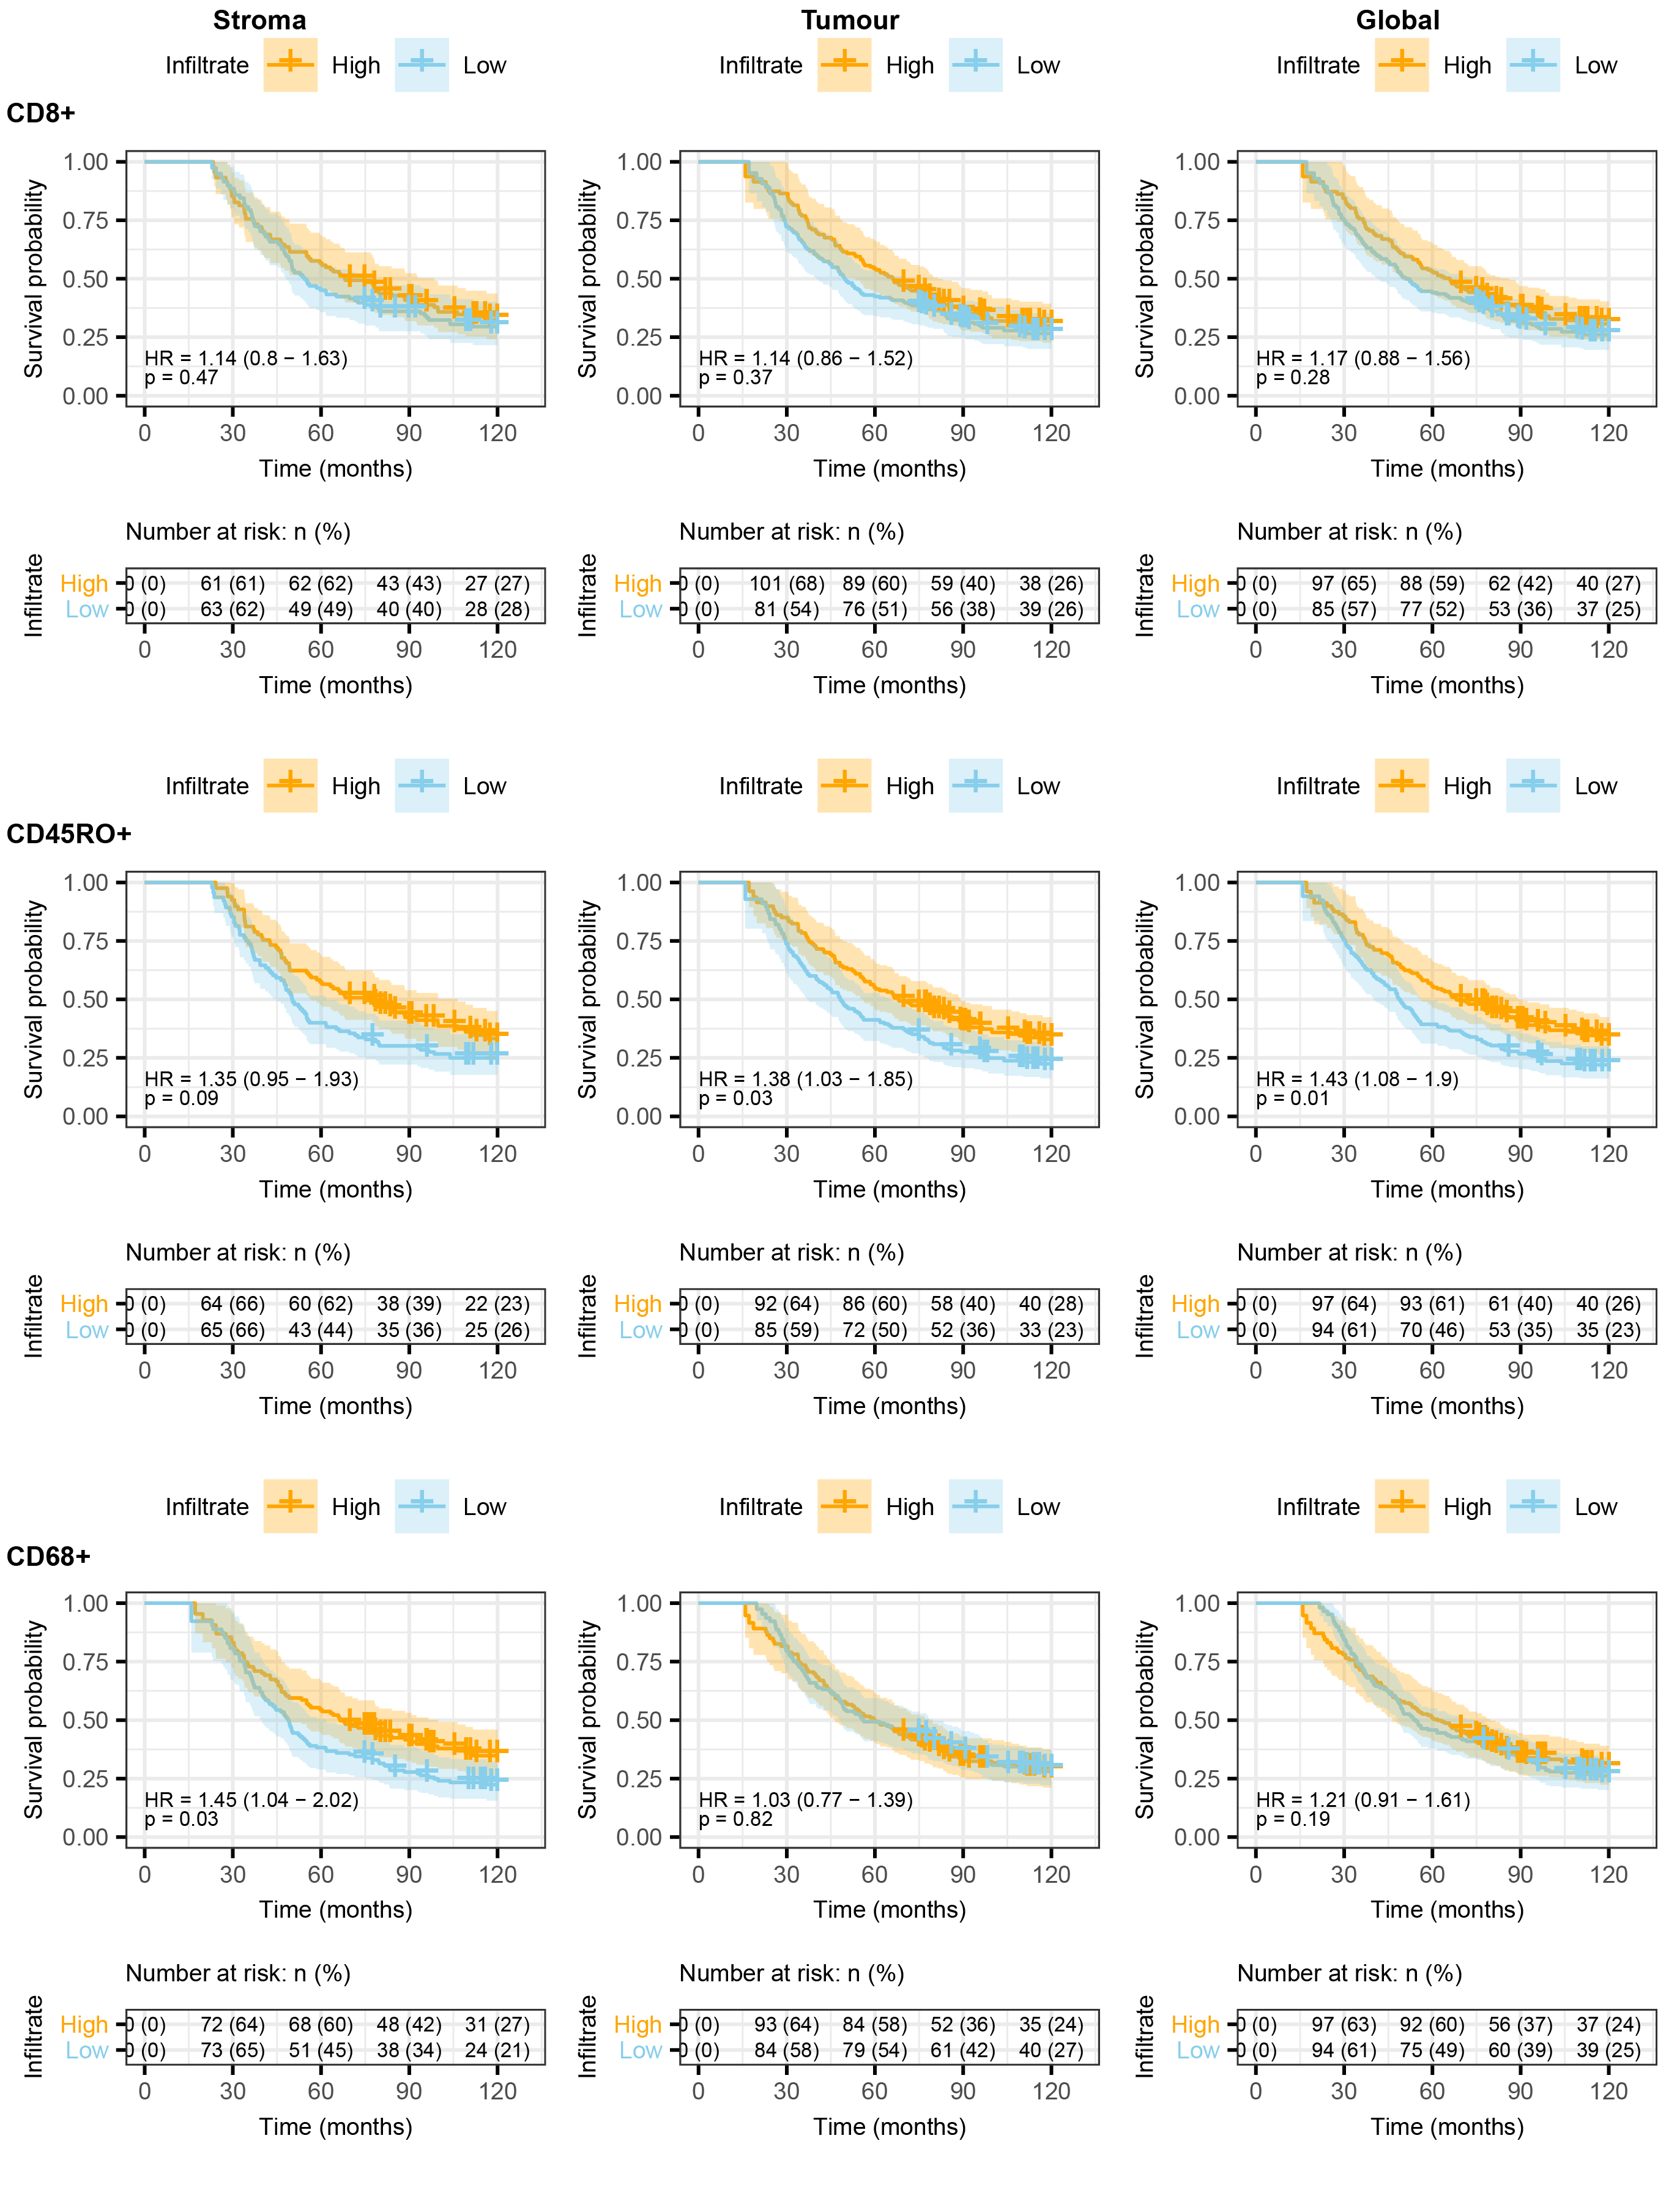
\includegraphics{Chapter2/Figs/Raster/KM_allinf.png}
    \caption[KM Survival curves for individual infiltrates]{Kaplan–Meier survival curves using cut point of median density of stromal CD68$^+$ macrophages and CD45RO$^+$ memory T cells using left truncation and right censoring. Median entry to the study for all patients after diagnosis was 26.4 months. Median follow up time from diagnosis to exit or death was 105.1 months.}
    \label{fig:KM_infiltrates}
\end{figure}


\subsection{Combined model}

Given that individually, all infiltrates were prognostic in at least one compartment, the next step was to model the survival of patients based on all infiltrates together to account for the different effects of differing infiltrates. I carried out multivariable Cox regression analysis including all infiltrates and stage on patients with complete data for all infiltrates (n=152) (Table \ref{tab:cox_combined}).  In this model only stage and CD68$^+$ stromal infiltrate were significant predictors of survival.

I then refined the model by removing the least significant elements (defined as those with p>0.1) (Table \ref{tab:cox_combined}, n=152). Interestingly, I found that the p-values for CD68$^+$ and CD45RO$^+$ stromal infiltrates in the refined model become less significant and the hazard ratios are attenuated in comparison to both the univariable regression and the full model. This is likely due to the inability of Cox regression to distinguish with confidence whether stromal CD45RO$^+$ or CD68$^+$ density is the most significant predictor when there is a strong correlation between all the immune variables.
\begin{table}[]
    \centering
    \begin{tabular}{llcccc} \hline
&&	Multivariable & (all combined) &	Refined model &\\ \hline
	&&	HR&	p-value&	HR&	p-value\\
CD8+&	Epithelium&	0.96&	0.81&	-	&-\\
	&Stroma&	1.07	0.63	&-&	-\\
CD45RO+&	Epithelium&	1.12&	0.37	&-&	-\\
	&Stroma	&0.83	&0.09	&0.68&	0.11\\
CD68+&	Epithelium&	1.16&	0.63	&-&	-\\
	&Stroma	&0.53&	0.038&	0.88	&0.17\\
Stage &&&&&\\
&Localised&	1&	0&	1&	0\\
&	Regional&	2.00&	0.16&	2.03&	0.14\\
&	Distant&	4.82&	<<0.001&	4.70&	0.0001\\
&	Unstaged	&8.15&	<<0.001&	8.25&	0.0001\\ \hline

    \end{tabular}
    \caption{}
    \label{tab:cox_combined}
\end{table}

\subsection{Ratio of stromal immune infiltrate to intra-epithelial immune infiltrate is not prognostic.}

Immune exclusion has been mentioned a lot and the location of immune infiltrate in either the intra-epithelial or stromal regions is a micro-environmental factor that can only be derived from images. The ratio of tumour to stromal infiltrate can be measured from images and may indirectly measure properties of the ECM that allow for infiltration into the tumour core or measure the extent of the interaction of the immune cells with epithelial cells. As shown previously, stromal and intra-epithelial immune cell densities are correlated. I investigated whether the ratio of stromal infiltrate density to intra-epithelial immune infiltrate density was a significant predictor of risk in HGSOC using the Cox proportional hazards model.

% latex table generated in R 3.3.2 by xtable 1.8-2 package
% Thu Oct 19 15:01:03 2017
\begin{table}[ht]
\centering
\begin{tabular}{rrrrrr}
  \hline
 & coef & exp(coef) & se(coef) & z & Pr($>$$|$z$|$) \\ 
  \hline
\multicolumn{5}{l}{

CD8$^+$
}\\
Stroma:Tumour ratio & 0.069 & 1.072 & 0.179 & 0.386 & 0.700 \\ 
 
\multicolumn{5}{l}{CD45RO$^+$
}\\
Stroma:Tumour ratio & -0.105 & 0.900 & 0.177 & -0.596 & 0.551 \\ 

\multicolumn{5}{l}{

CD68$^+$
}\\
Stroma:Tumour ratio & 0.010 & 1.010 & 0.005 & 1.772 & 0.076 \\ 
   \hline
\multicolumn{5}{l}{}\\
\end{tabular}
\caption[Cox regression for ratio of Tumour to Stroma infiltrate]{Single predictor Cox proportional hazard tests with ratios of stromal to tumour infiltrate as predictors.} 
\label{tab:s:t}
\end{table}
There is no significant effect on survival of stroma:tumour ratio for any of the infiltrates. It is worth noting that the subset of evaluable patients included here decreases. This is because only cores with non zero tumour infiltrate density can be included. I would have expected that the quantity of infiltration from the stromal to intra-epithelial regions would have effected tumour progression and hence survival so this is an interesting negative result.

\subsection{Principal components of the combined immunospace describe biologically interpret-able effects.}
 Part of the problem that I encountered in analysing the effect of multiple immune populations upon survival is that the multiple immune infiltrates are correlated (see Figure \ref{fig:ch2_correlation}) and may have additive or suppressive effects.  In order to assess the multi-dimensional nature of the immune response in more detail I proposed that as the three types of immune infiltrate vary continuously across epithelium and stroma these variables can be regarded as six dimensions of an ‘immunospace’ (three infiltrates, 2 localizations).  Given the strong correlations between infiltrates (Figure \ref{fig:ch2_correlation}), we can safely say these immune variables are not independent. I used principal component analysis (PCA) to determine the independent patterns across these dimensions, using the 152 patients for whom complete data were available.
 
 PCA transformed the six correlated infiltrate variables into six independent axes with the first component containing the largest proportion of variance (60\%) in the data set\ref{tab:PC}. In principal component 1 (PC1), the weightings of all immune infiltrates are positive and similar in magnitude (Table \ref{tab:PC}). This indicates that as one infiltrate increases so do all the others and represents the degree of coordinated immune response. The remaining principal components characterize additional patterns across immune infiltrates independent of PC1. The additive contribution of PC2 characterises negative correlation between CD8$^+$ infiltrates and CD68$^+$ macrophages and CD45RO$^+$ memory cells. PC3 characterizes additional variation where epithelial and stromal infiltrates are negatively correlated, the most positive values of PC3 correspond to high infiltration in tumour epithelium compared to stroma and the most negative values of PC3 correspond to the opposite, the aforementioned immune exclusion. 
 
\begin{table}[]
    \centering
    \begin{tabular}{lllllll}
&PC1& PC2&PC3&PC4&PC5&PC6\\
\hline
CD8$^+$ tumour density& 0.38&-0.56&0.58&-0.1&0.4&-0.21\\
CD8$^+$ stromal density&0.38&-0.59&-0.47&0.27&-0.21&0.43\\
CD68$^+$ tumour density&0.41&0.47&0.37&0.11&0.09&0.67\\
CD68$^+$ stromal density&0.42&0.3&-0.29&0.56&0.36&-0.45\\
CD45RO$^+$ tumour density&0.45&0.11&0.21&-0.07&-0.78&-0.36\\
CD45RO$^+$ stromal density&0.41&0.15&-0.42&-0.77&0.22&-0.03\\
\hline
    \end{tabular}
    \caption{Contributions of normalized infiltrates to all principal components.}
    \label{tab:PC}
\end{table}


 
Having calculated the principal components from the data, it is possible to extract the patients who lie at the most extreme ends of these axes of variation. Figure \ref{fig:PC_examples} shows representative images with the largest magnitudes of PC1, PC2 and PC3 to visually illustrate the patterns described above. The variance in the remaining principal components (4-6) is smaller and less informative. Variance in PC4 is predominantly from CD45RO$^+$ stromal density, PC5 is from CD45RO$^+$ epithelial density and PC6 is from CD68$^+$ epithelial density. Patients are plotted by their PC1 and PC2 values in \ref{fig:PC_plot}. 
In order to evaluate the prognostic impact of these patterns of infiltration, I used Cox proportional hazard regression to assess whether these principal components were predictive of survival. Cox regression survival models were also calculated on all combinations of principal components and stage. Only PC1 was an independent predictor of survival in this cohort and was associated with improved survival (Univariate: HR=$0.89$, $p=0.024$, PC1+Stage: HR: $0.88$, $p=0.019$) (Table \ref{tab:pc_surv}) reflecting the good prognosis of a strong coordinated immune response. The association of this principal component with survival is also illustrated graphically using Kaplan Meier curves in Fig. \ref{fig:km_PC}.
\begin{landscape}
\begin{figure}[width=0.8\textwidth, keepaspectratio]
    \centering
    \includegraphics[width=\textwidth]{Chapter2/Figs/Raster/PC_montfort.png}
    \caption[Examples of tissue sections with largest values of principal components.]{Images of the sections of patients with the highest values of principal components 1, 2 and 3. The values of the immune infiltrates of these images are shown on the boxplots of the distribution across all samples.}
    \label{fig:PC_examples}
\end{figure}
\end{landscape}

\begin{figure}
    \centering
    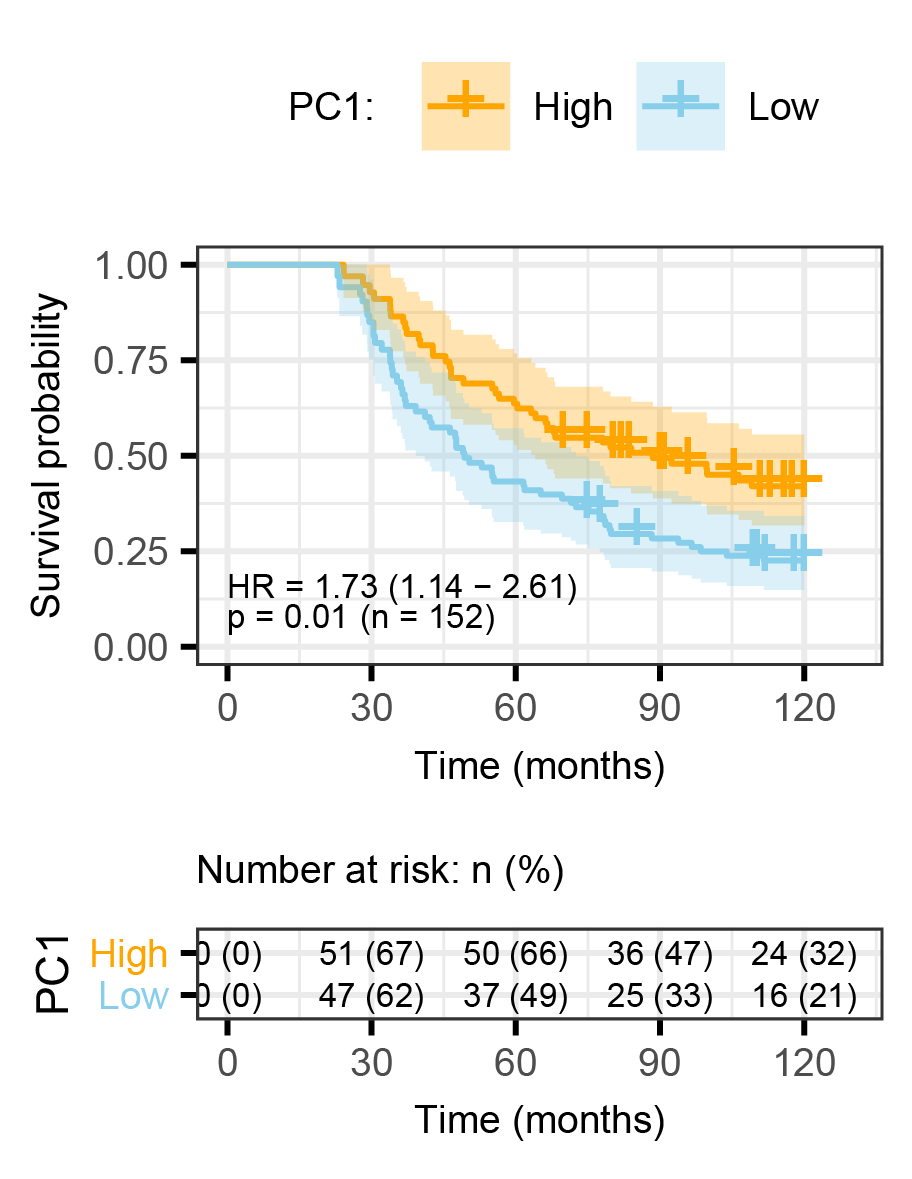
\includegraphics{Chapter2/Figs/Raster/Montfort-2018_Fig7A-PC1.png}
    \caption[Kaplan Meier Curves for Principal Component 1]{Kaplan Meier illustrative survival curve. Principal component 1 are split at the median. The survival of high and low values of Principal component 1 are plotted against time. }
    \label{fig:km_PC}
\end{figure}

\subsection{Comparing Survival Models}
 The Akaike Information Criterion (AIC) was used to compare the performance of these survival models and includes a penalty on the number of terms to reduce over-fitting (Supplementary Fig. 8). The model combining stage, PC1 and PC5 had the best performance for predicting overall survival. The improvement with the addition of PC5 shows that the addition of this principal component has a suppressor effect in the model, increasing the significance of other variables when included. This demonstrates that survival is predominantly determined by the coordinated immune response and further variation in survival from this trend can be encoded by the quantity of epithelial CD45RO$^+$ infiltrate. Interestingly, the models that contained stage and either stromal CD45RO$^+$ or CD68$^+$ infiltrate contained a similar amount of information about patient survival as the one that contained stage and principal components 1 and 5. In our cohort, the density of CD68$^+$ and CD45RO$^+$ stromal infiltrates are therefore the best single infiltrates for survival modelling. 
 
 \begin{figure}
     \centering
     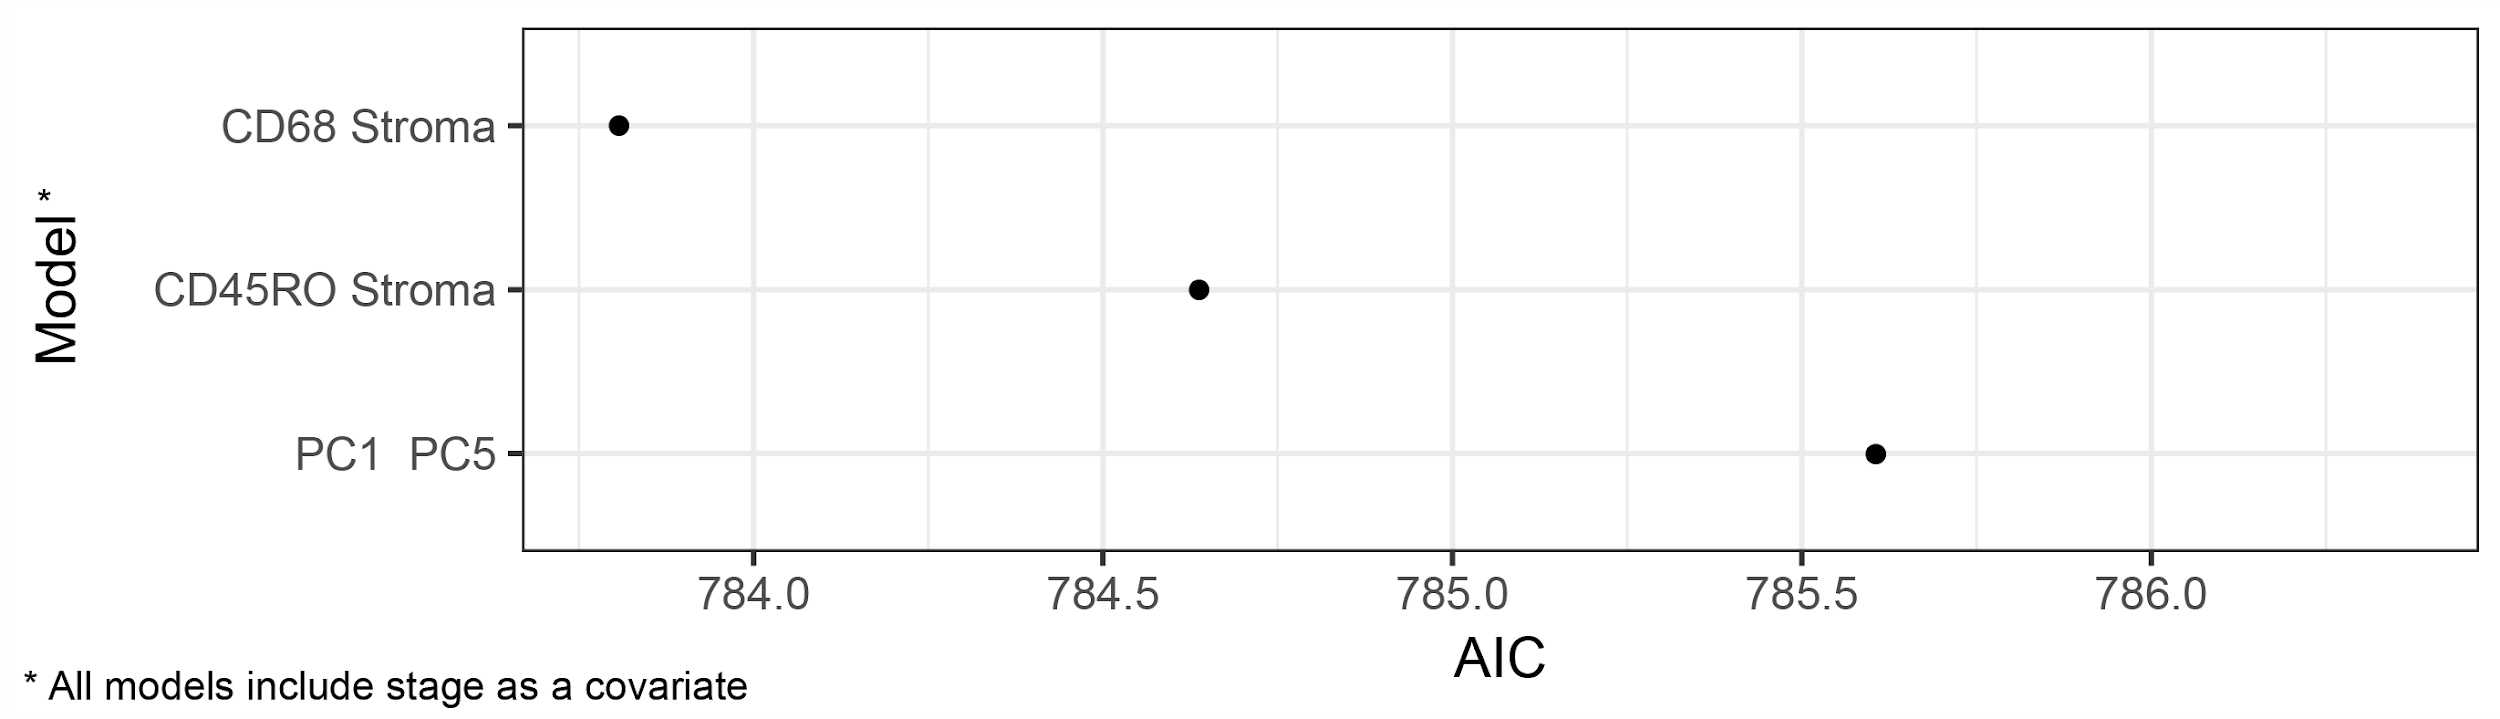
\includegraphics{AIC}
     \caption{AIC for most significant models (AIC > 2)}
     \label{fig:AIC}
 \end{figure}


\subsection{Are genetic defects associated with HGSOC driving individual infiltrates or the coordinated immune response in tumours?}

\subsubsection*{Infiltrate density is not significantly associated with \textit{BRCA} status}
To investigate the interactions between the TME and the genome, can ask whether a germline mutation in either of the \textit{BRCA1/2} genes results in changes in the TME and specifically the immune infiltrate. I investigated whether tumour, stroma or full core measures of CD8$^+$, CD45RO$^+$or CD68$^+$densities were related to \textit{BRCA1/2} mutations using the Kruskal-Wallis rank sum test. I compared the infiltrate density distributions between patients with no mutation, a mutation in \textit{BRCA1} and a mutation in \textit{BRCA2}. I found that the distributions of CD8$^+$, CD45RO$^+$and CD68$^+$infiltrates and the principal components were not significantly associated with \textit{BRCA} mutation status (Figure \ref{fig:genomic}). This was unexpected as previous results have found increases in CD8$^+$infiltrate with a \textit{BRCA1} mutation\cite{Clarke2009}.

\subsubsection{Infiltrate density is not significantly associated with type of \textit{TP53} mutation.}
Mutant P53 proteins have been linked to multiple micro-environmental changes\cite{Cordani2016}. I investigated whether the type of TP53 mutation produced measurable changes in the TME. Tumour, stroma or full core measures of CD8$^+$, CD45RO$^+$or CD68$^+$densities were compared between gain or loss of function mutations in \textit{TP53}. I used the Kruskal-Wallis rank sum test and found that the distribution of immune infiltrate was not significantly associated with type of \textit{TP53} mutation.

\subsubsection{Infiltrate density is not significantly associated with change in PTEN expression.}
Changes in PTEN expression are cell-intrinsic and levels of PTEN expression are prognostic in HGSOC\cite{RN17, RN15}. Tumour, stroma or full core measures of CD8$^+$, CD45RO$^+$ or CD68$^+$ densities were compared between patients with high or low PTEN expression as measured by both IHC and IF. Using the Kruskal-Wallis rank sum test I found that change in PTEN expression was not significantly associated with any change in the density of immune infiltrate. This particular cell-intrinsic change is not associated with a change in immune infiltration in our cohort.

The presence of germline \texit{BRCA2} mutations was significantly associated with lower CD8$^+$ cell density than patients with a \texit{BRCA1} after multiple testing correction (Figure \ref{fig:genomic}). There was no significant association between the quantity of CD45RO$^+$ or CD68$^+$ infiltrate and the mutational status of either \texit{BRCA1} or \texit{BRCA2} genes (Figure \ref{fig:genomic}) . No significant association was detected between TP53 GOF and LOF mutations or PTEN expression and the densities of CD8$^+$, CD45RO$^+$ and CD68$^+$ cells in epithelium or stroma (Table \ref{tab:}). Similarly, changes in the principal components were not significantly associated with PTEN expression, TP53 GOF or LOF mutation or germline \textit{BRCA1}/\texit{BRCA2} mutation status (Table \ref{tab:}). 

\begin{figure}
    \centering
    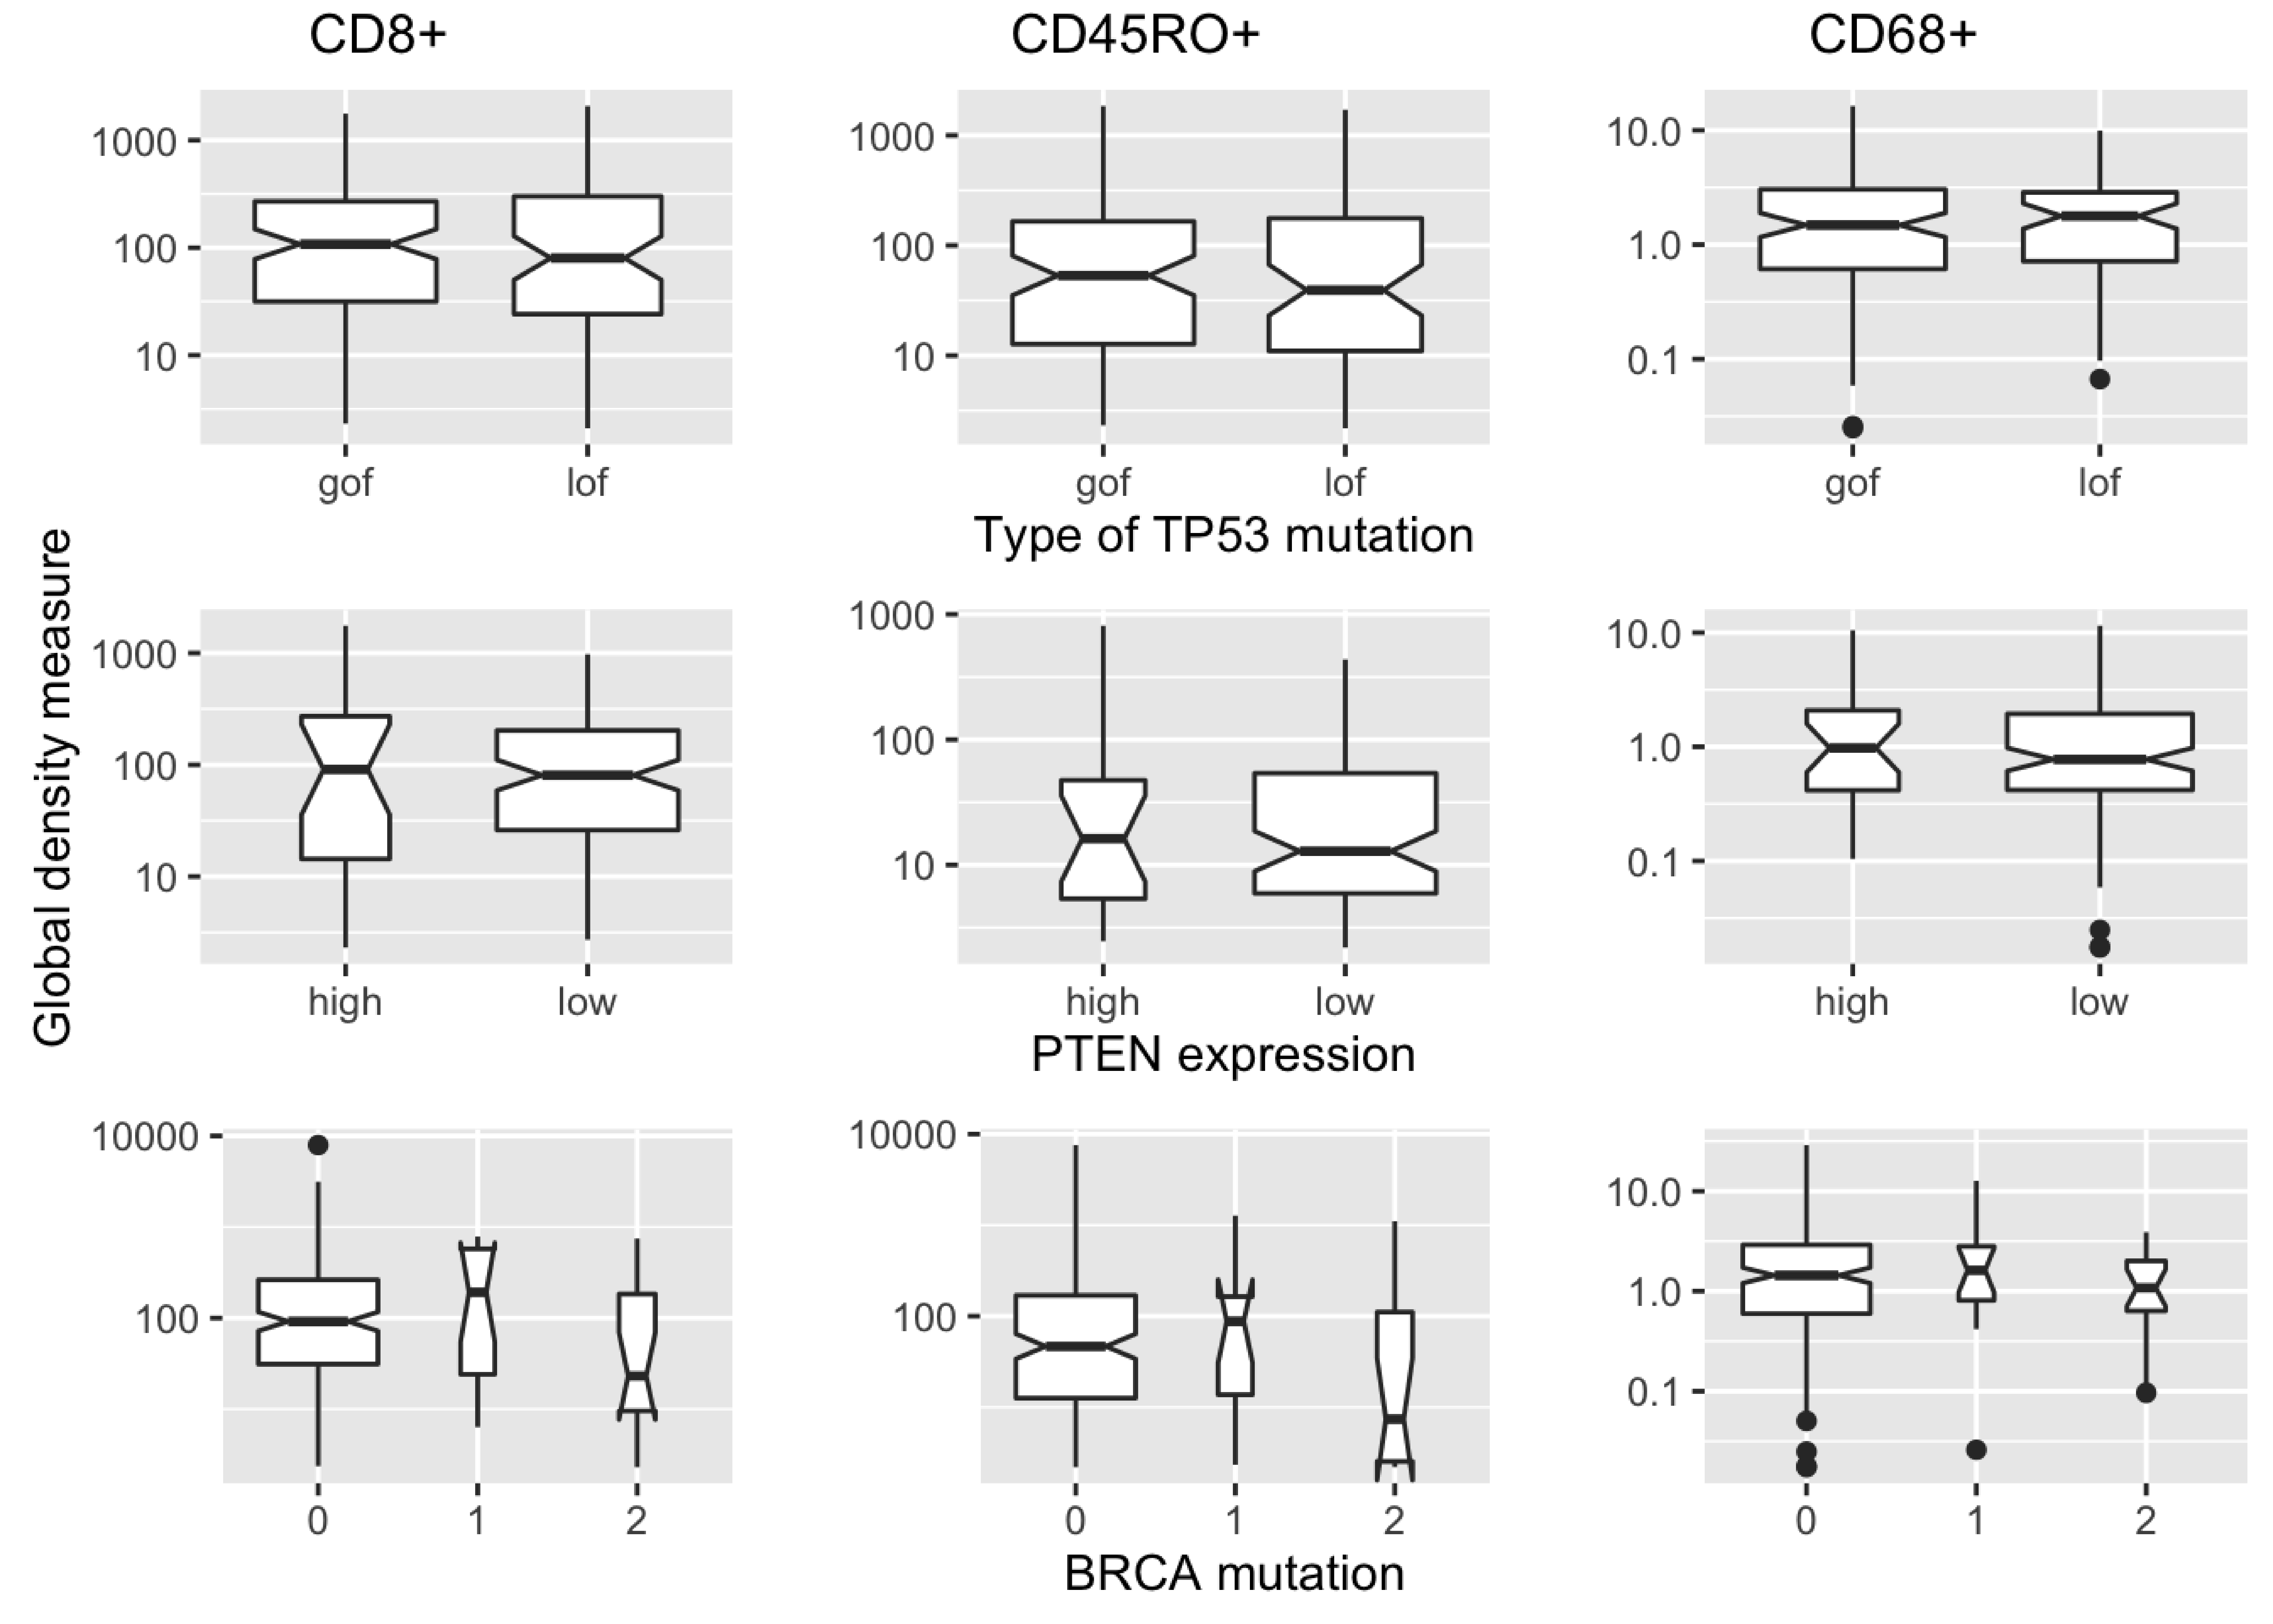
\includegraphics[width=\textwidth]{Chapter2/Figs/Raster/genomic.png}
    \caption{Boxplots of Infiltrate distribution against genomic phenotype.}
    \label{fig:genomic}
    
\end{figure}


\begin{table}[]
    \centering
    \begin{tabular}{c|c}
         &  \\
         & 
    \end{tabular}
    \caption{T-test for association between PTEN, BRCA status or GOF/LOF mutations and immune infiltrate }
    \label{tab:my_label}
\end{table}

\subsection{Other ovarian cancer subtypes}

\begin{figure}
    \centering
    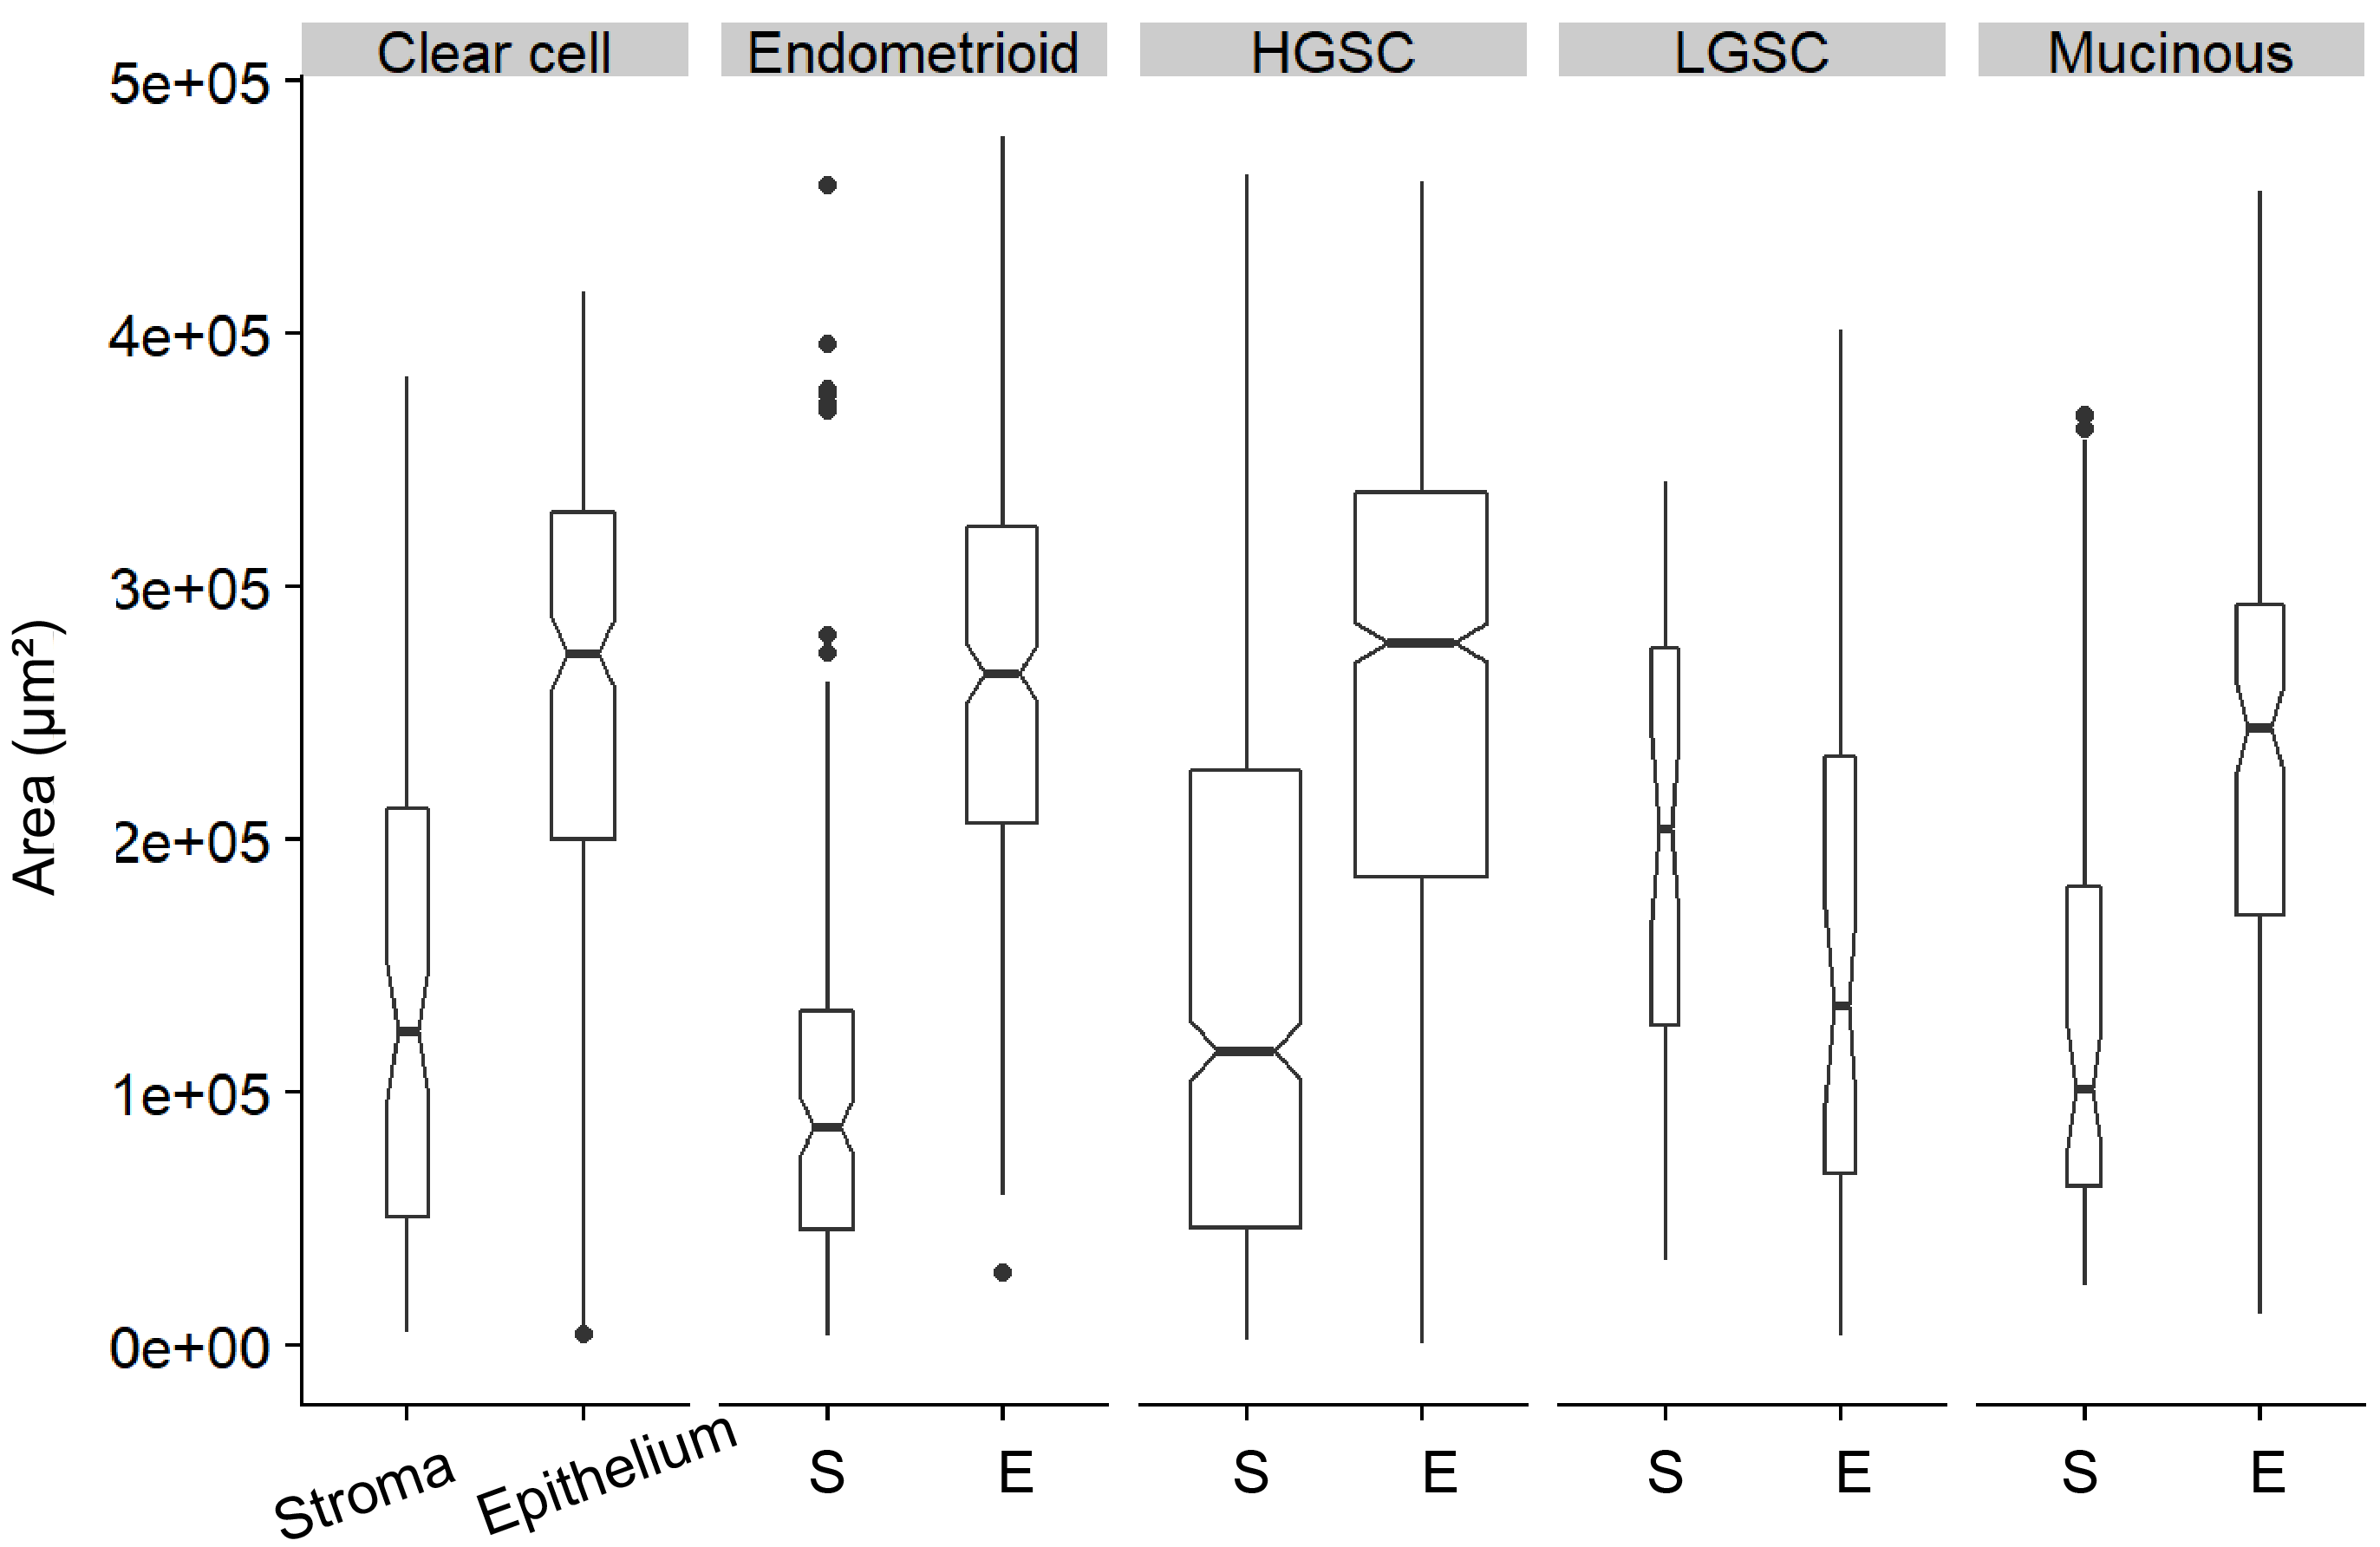
\includegraphics[width=0.8\textwidth]{Chapter2/Figs/Raster/Morphology_area.png}
    \caption{Area of tumour and stroma across morphological subtypes.}
    \label{fig:morph_area}
\end{figure}

\clearpage

\section{Discussion}
 One of the key and novel findings of this work was that the global measure of CD8$^+$ infiltrate was a stronger and more significant predictor of survival over CD8$^+$ infiltrate alone. The implication of the average infiltration being a stronger predictor of survival is that averaging over the intra-tumour stroma allows for a better measure of long term infiltration dynamics and measures the presence of a reservoir of immune cells, poised to infiltrate the epithelium.  I also demonstrated here that the quantity of epithelial and stromal CD45RO$^+$ is a positive prognostic feature, a result which also confirms the positive incremental benefit of a long term and mature immune response. 
 
 I observed in addition that stromal and epithelial populations and all infiltrates were somewhat positively correlated. It is worth noting that the  CD8$^+$ and  CD45RO$^+$ subpopulations are not biologically mutually exclusive and as such I expect some correlation between quantities but in this dataset there was no opportunity to examine the specific spatial locations of the immune cells. 

As discussed in the introduction, many pieces of research have illustrated that macrophage function is micro-environment dependent\cite{ZhangMacrophage2014, li2018intratumoral}, demonstrating that exact localisation effects macrophage function. My work is in agreement with the observation by Li et al. that stromal regions are most prognostic in which to evaluate macrophages. I find however, in contrast to their work in lung cancer, that CD68$^+$ macrophages are a positive prognostic feature. Further elucidation of the nature of macrophages and their interaction with the TME is required and some such questions are investigated in this thesis.
These observations all suggest that despite the focus of many studies being the intra-epithelial immune infiltration, perhaps due to a focus on direct contact and cytotoxic interaction between immune and tumour cells, that stromal infiltrate should be evaluated. It appears that stromal infiltration plays its own role in the immune response as well as perhaps providing more information about the epithelial infiltration through inference of long term immune infiltration dynamics.

In this chapter I also developed the idea of an immunospace by viewing the quantity of each immune infiltration as part of a multidimensional immune landscape. This approach allowed me to analyse patterns across different immune populations and to derive the principal components as measures of variation. I observed that the correlation between infiltrates amounts to general coordinated immune response which is a positive prognostic. It also allowed me to examine the independence of other phenomenon as the immune exclusion from the epithelium which could be obtained in an unbiased manner.

Using quantitative data also allowed me to define a threshold for immune exclusion, a 10 fold difference in immune infiltration. I observed that CD8$^+$,  CD45RO$^+$ and  CD68$^+$  infiltrates predominantly exist on a continuum without clear justification for cutpoints.

This work also finds no link between immune infiltration and germline \textit{BRCA} mutations, this is in part due to effects of cohort size. With approximately 20 patients with mutations, I am underpowered to ask multiple questions about the differences in immune infiltration between non-\textit{BRCA} and \textit{BRCA}-mutated patients.

The exact spatial nature of immune infiltration when taking into account tumour structure is unknown. There may also be a link between stromal immune infiltration and collagen deposition. Comparisons of immune infiltration to that which would be expected from diffusion into the epithelium alone has not been examined and is a key questions in the rest of this thesis.

